\documentclass[a4paper, 11pt]{article}
\usepackage[utf8]{inputenc} % Change according your file encoding
\usepackage{graphicx}
\usepackage{url}

%opening
\title{Seminar Report: Paxy}
\author{Maria Gabriela Valdes and Victoria Beleuta}
\date{\today{}}

\begin{document}

\maketitle

\section{Introduction}

This assignment gave us the opportunity to learn and implement the \textit{Paxos} algorithm. This algorithm is a protocol for solving consensus between processes in a distributed system. Consensus consists in agreeing on a proposed value among a group of participants. In this particular case, we have a set of \textit{Proposers} that propose different values, to a set of \textit{Acceptors} until a single and unique value is agreed between all \textit{Proposers} and \textit{Acceptors}.

\section{Work done}

We have completed the code files provided to correctly implement the algorithm. Our source code consists of two folders: \textit{src} and \textit{src-sep}. The first one contains the \textit{Erlang} files implementing the \textit{Paxos} algorithm with both groups of proposers and acceptors starting in the same \textit{Erlang} environment. In the folder \textit{src-sep} we have modules to give the possibility to start the group of proposers and the acceptors in two different \textit{Erlang} nodes.\\

To start the algorithm locally you have to call the function \textit{start} of module \textit{paxy} with only one argument, a list of int values of the same size of the number of proposers used. Each value represents the initial sleep time of each proposer (in milliseconds). For example: \\

\textit{paxy:start([2000,2000,2000]).}\\

With this command the \textit{Paxos} algorithm will start with three proposers, each one with 2 seconds of initial sleep, and five acceptors. Both group of proposers and acceptors will start in the same \textit{Erlang} node.\\

To start the algorithm with proposers and acceptors both in different \textit{Erlang} nodes you first have to start two different \textit{Erlang} environments. For example:\\

\begin{itemize}

\item In one terminal type \textit{erl -sname proposers}. This will represent an \textit{Erlang} node name \textit{proposers@server}.

\item In another different terminal type \textit{erl -sname acceptors}. This will represent a \textit{Erlang} node name \textit{acceptors@server}.

\end{itemize}

To start the proposers you have to call the function \textit{start\_sep\_proposers} of module \textit{paxy\_sep} with two arguments, a list of int values of the same size of the number of proposers used, the same as explained before, and the name of the acceptor's node, in the previous example named \textit{acceptors@server}. This command has to be called from the proposers's node. For example: \\

\textit{paxy\_sep:start\_sep\_proposers([2000,2000,2000], acceptors@server).}\\

In a similar way to start the acceptors you have to call the function \textit{start\_sep\_acceptors} of module \textit{paxy\_sep} with one argument, the name of the proposer's node, in the previous example named \textit{proposers@server}. This command has to be called from the acceptors's node. For example: \\

\textit{paxy\_sep:start\_sep\_acceptors(proposers@server).}\\

With this command the \textit{Paxos} algorithm will start with 3 proposers, each one with 2 seconds of initial sleep, and 5 acceptors. Both group of proposers and acceptors will start in different \textit{Erlang} nodes.

\section{Experiments}

First we run an experiment in the same machine with 3 proposers and 5 acceptors. After compiling the code files located in \textit{src} and running the paxy module \textit{paxy:start([200,200,200])}. Proposer 0, \textit{willard} proposes color \textit{blue}, and in round 2, the acceptors voted for \textit{kilgore} and decided on color \textit{blue}.\\

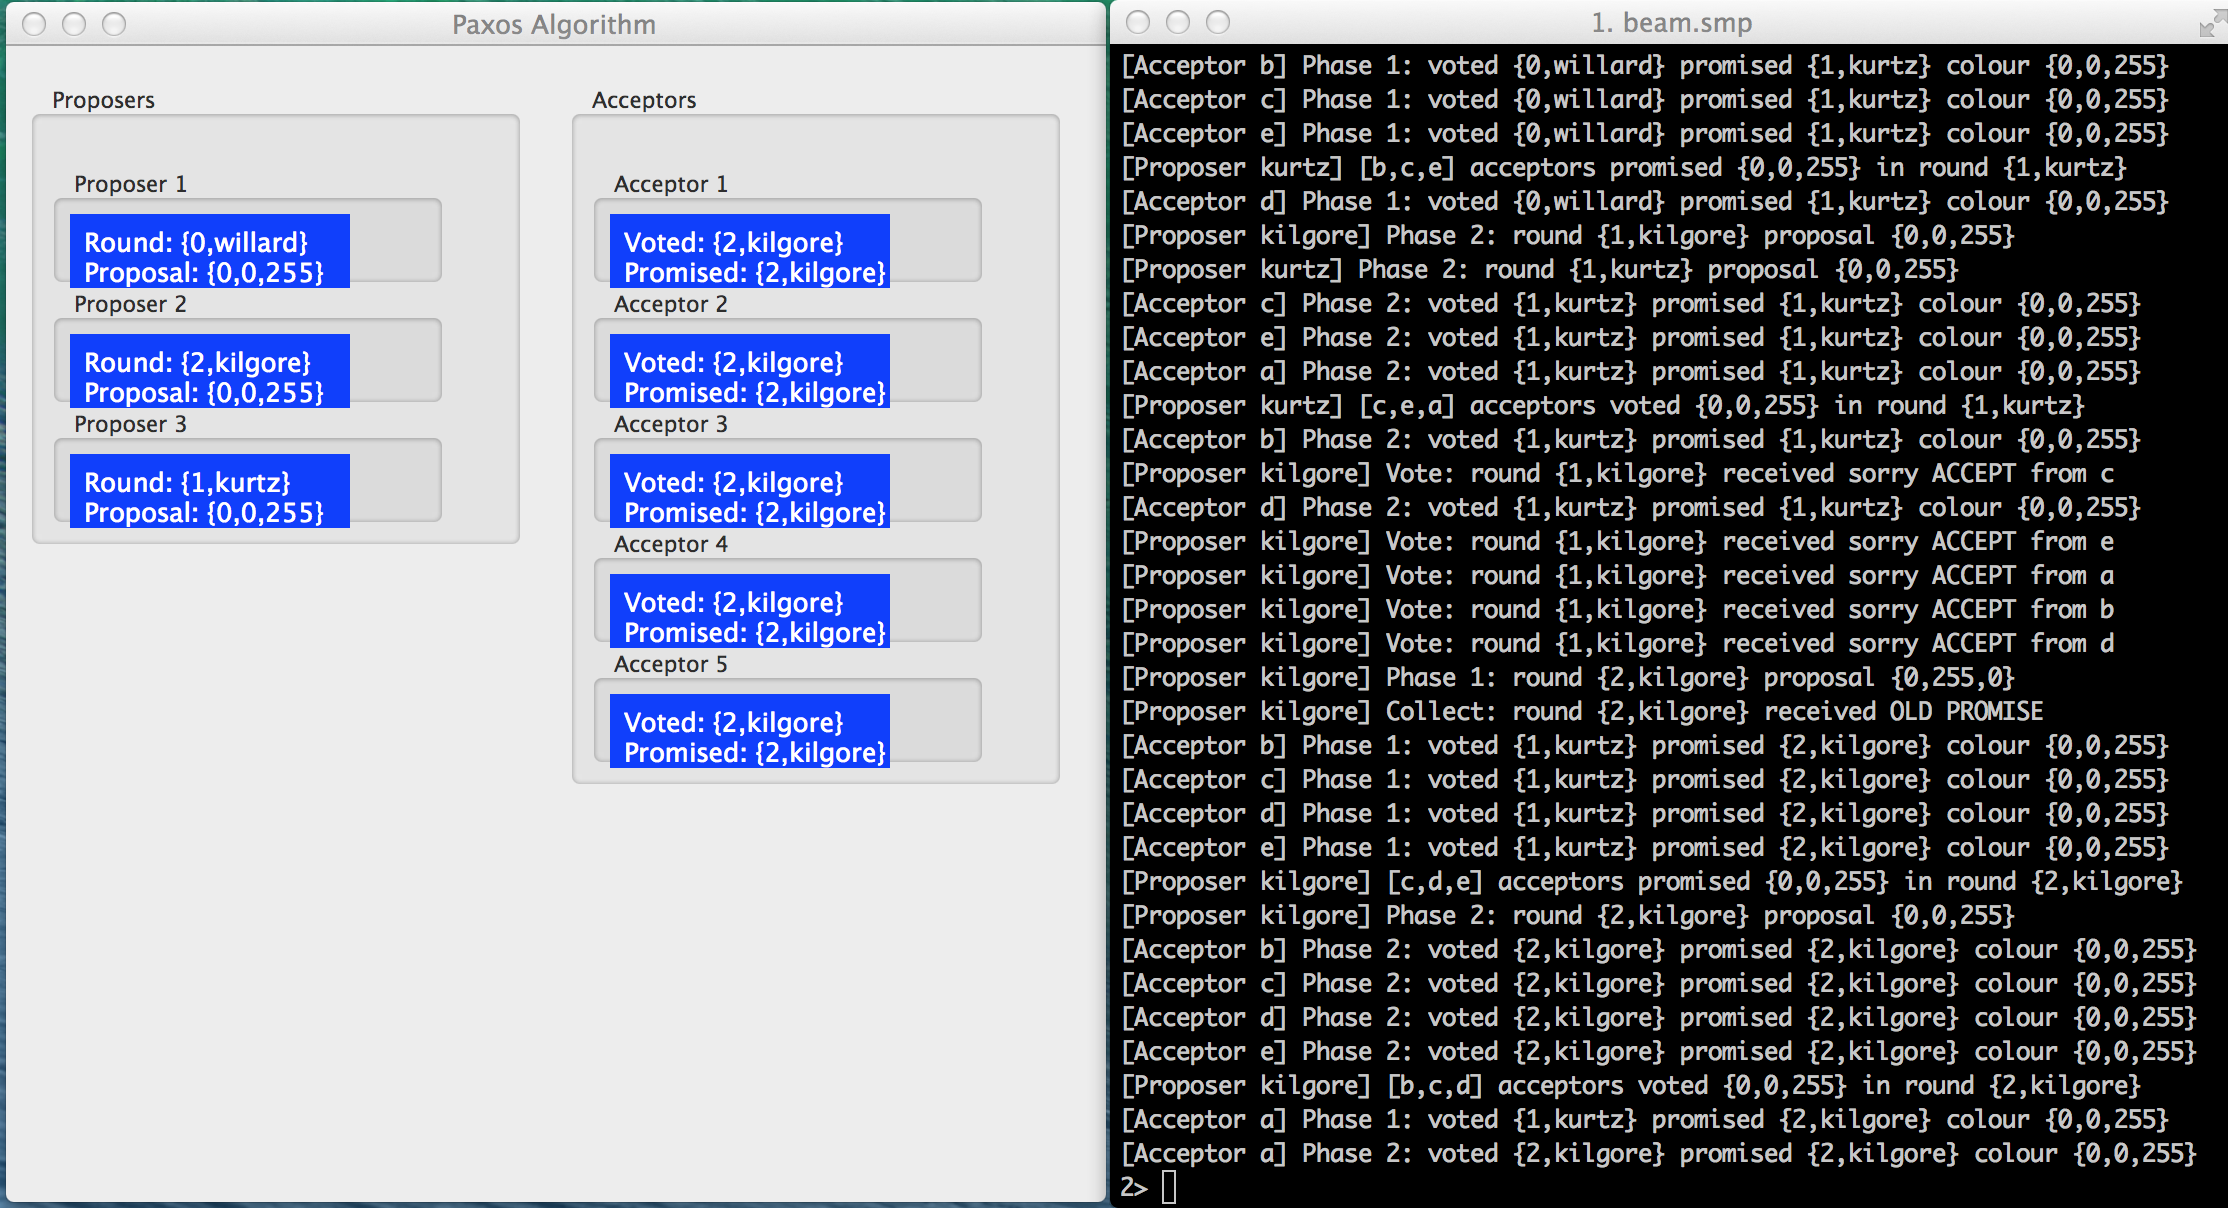
\includegraphics[scale=0.35]{images/exp0.png} \\\\

\textbf{i)} In this experiment we delay \textit{prepare} messages before sending them to proposers and we see that the algorithm terminates even with the delays shown in the trace.\\

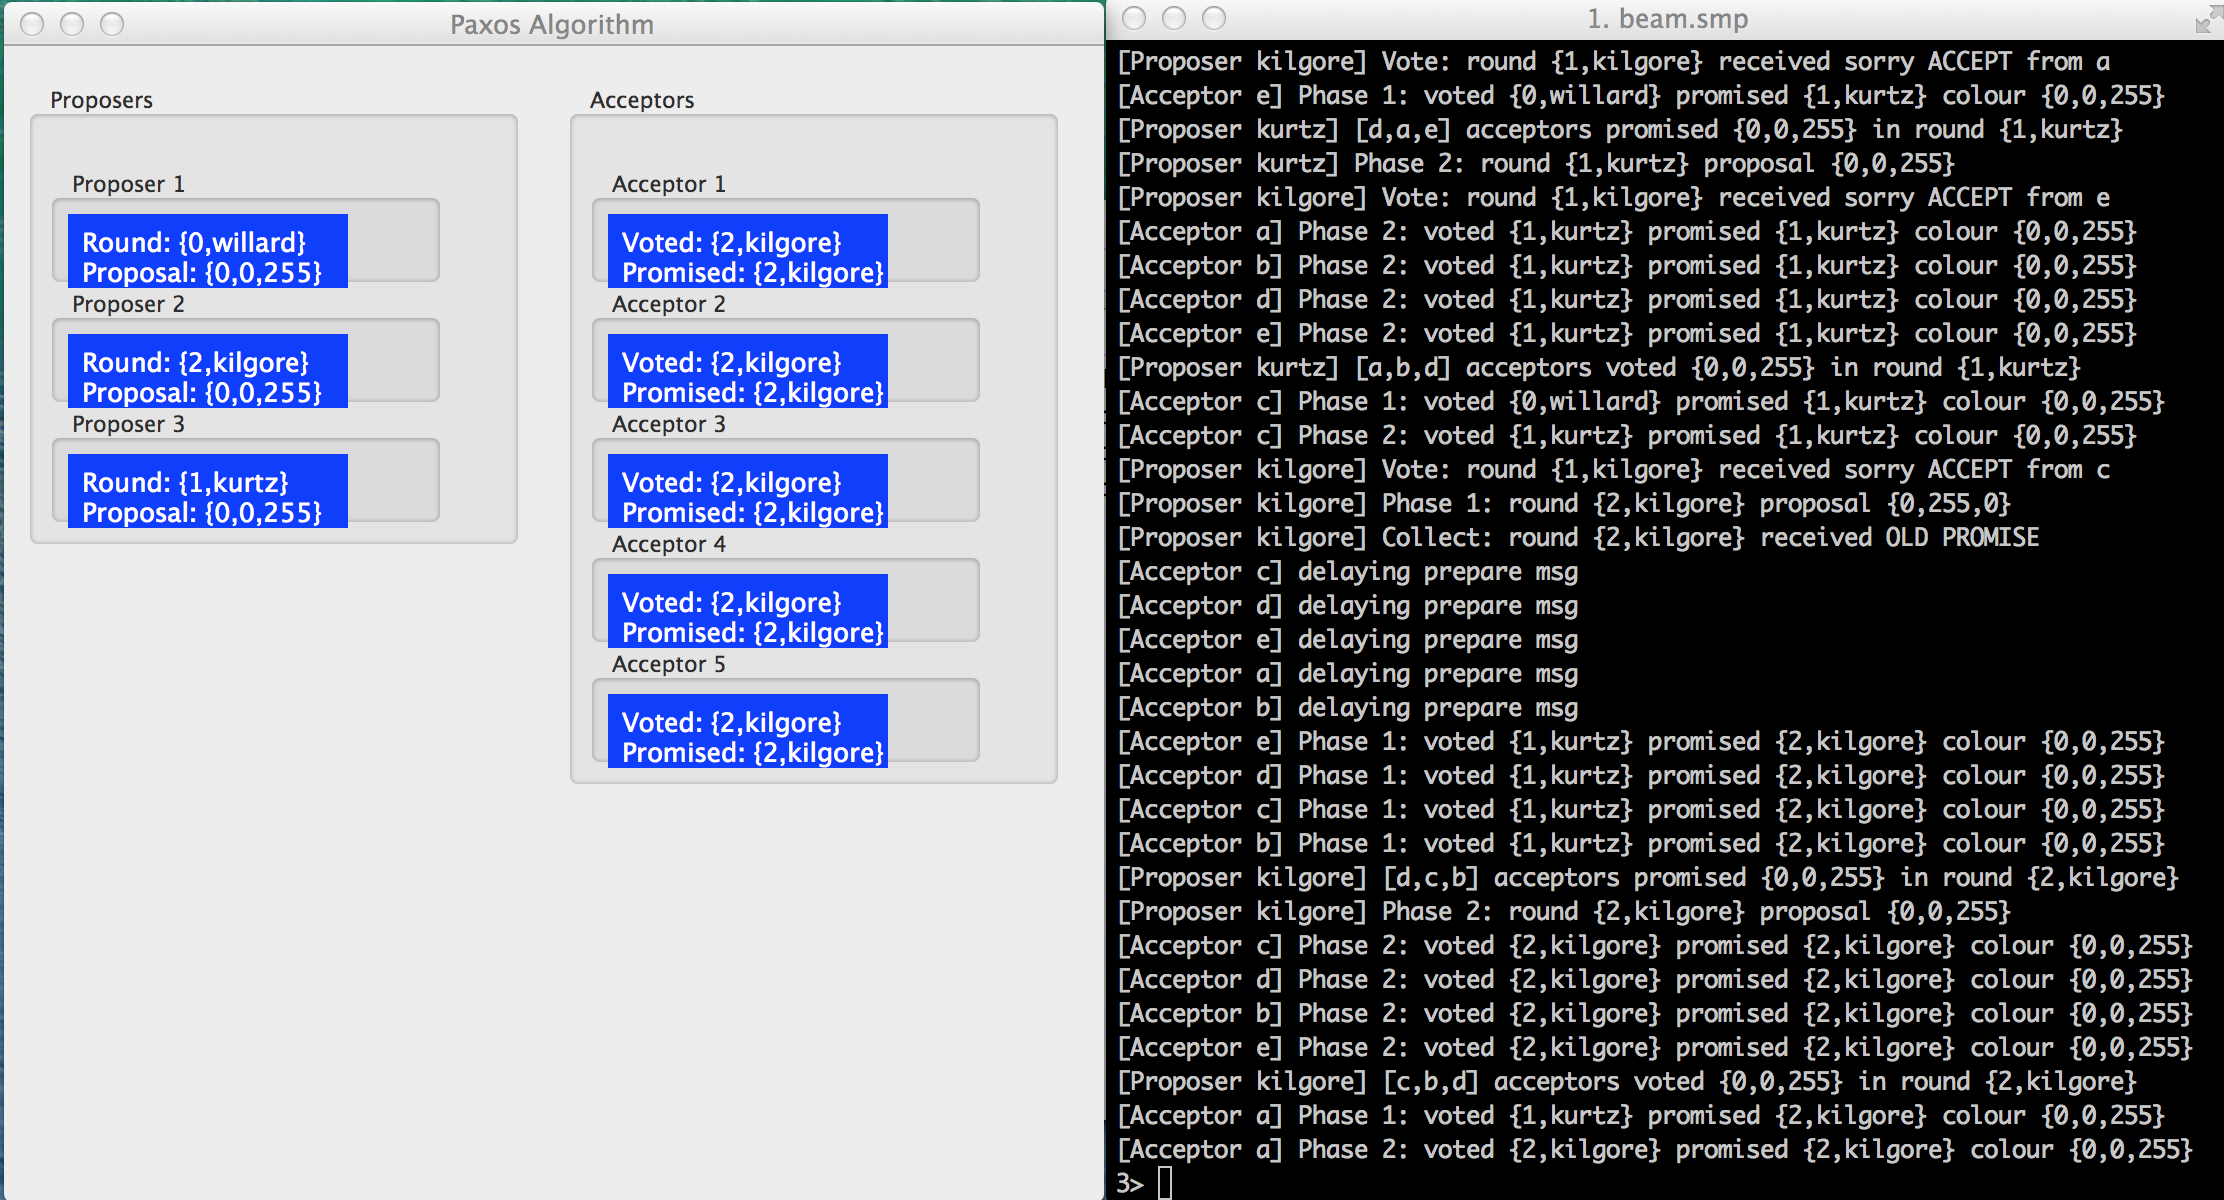
\includegraphics[scale=0.35]{images/exp1.png} \\\\
\newpage

Now we add delays before the \textit{accept} messages are sent to proposers, the algorithm terminates voting in round 2 for \textit{kilgore} and color \textit{blue}.\\

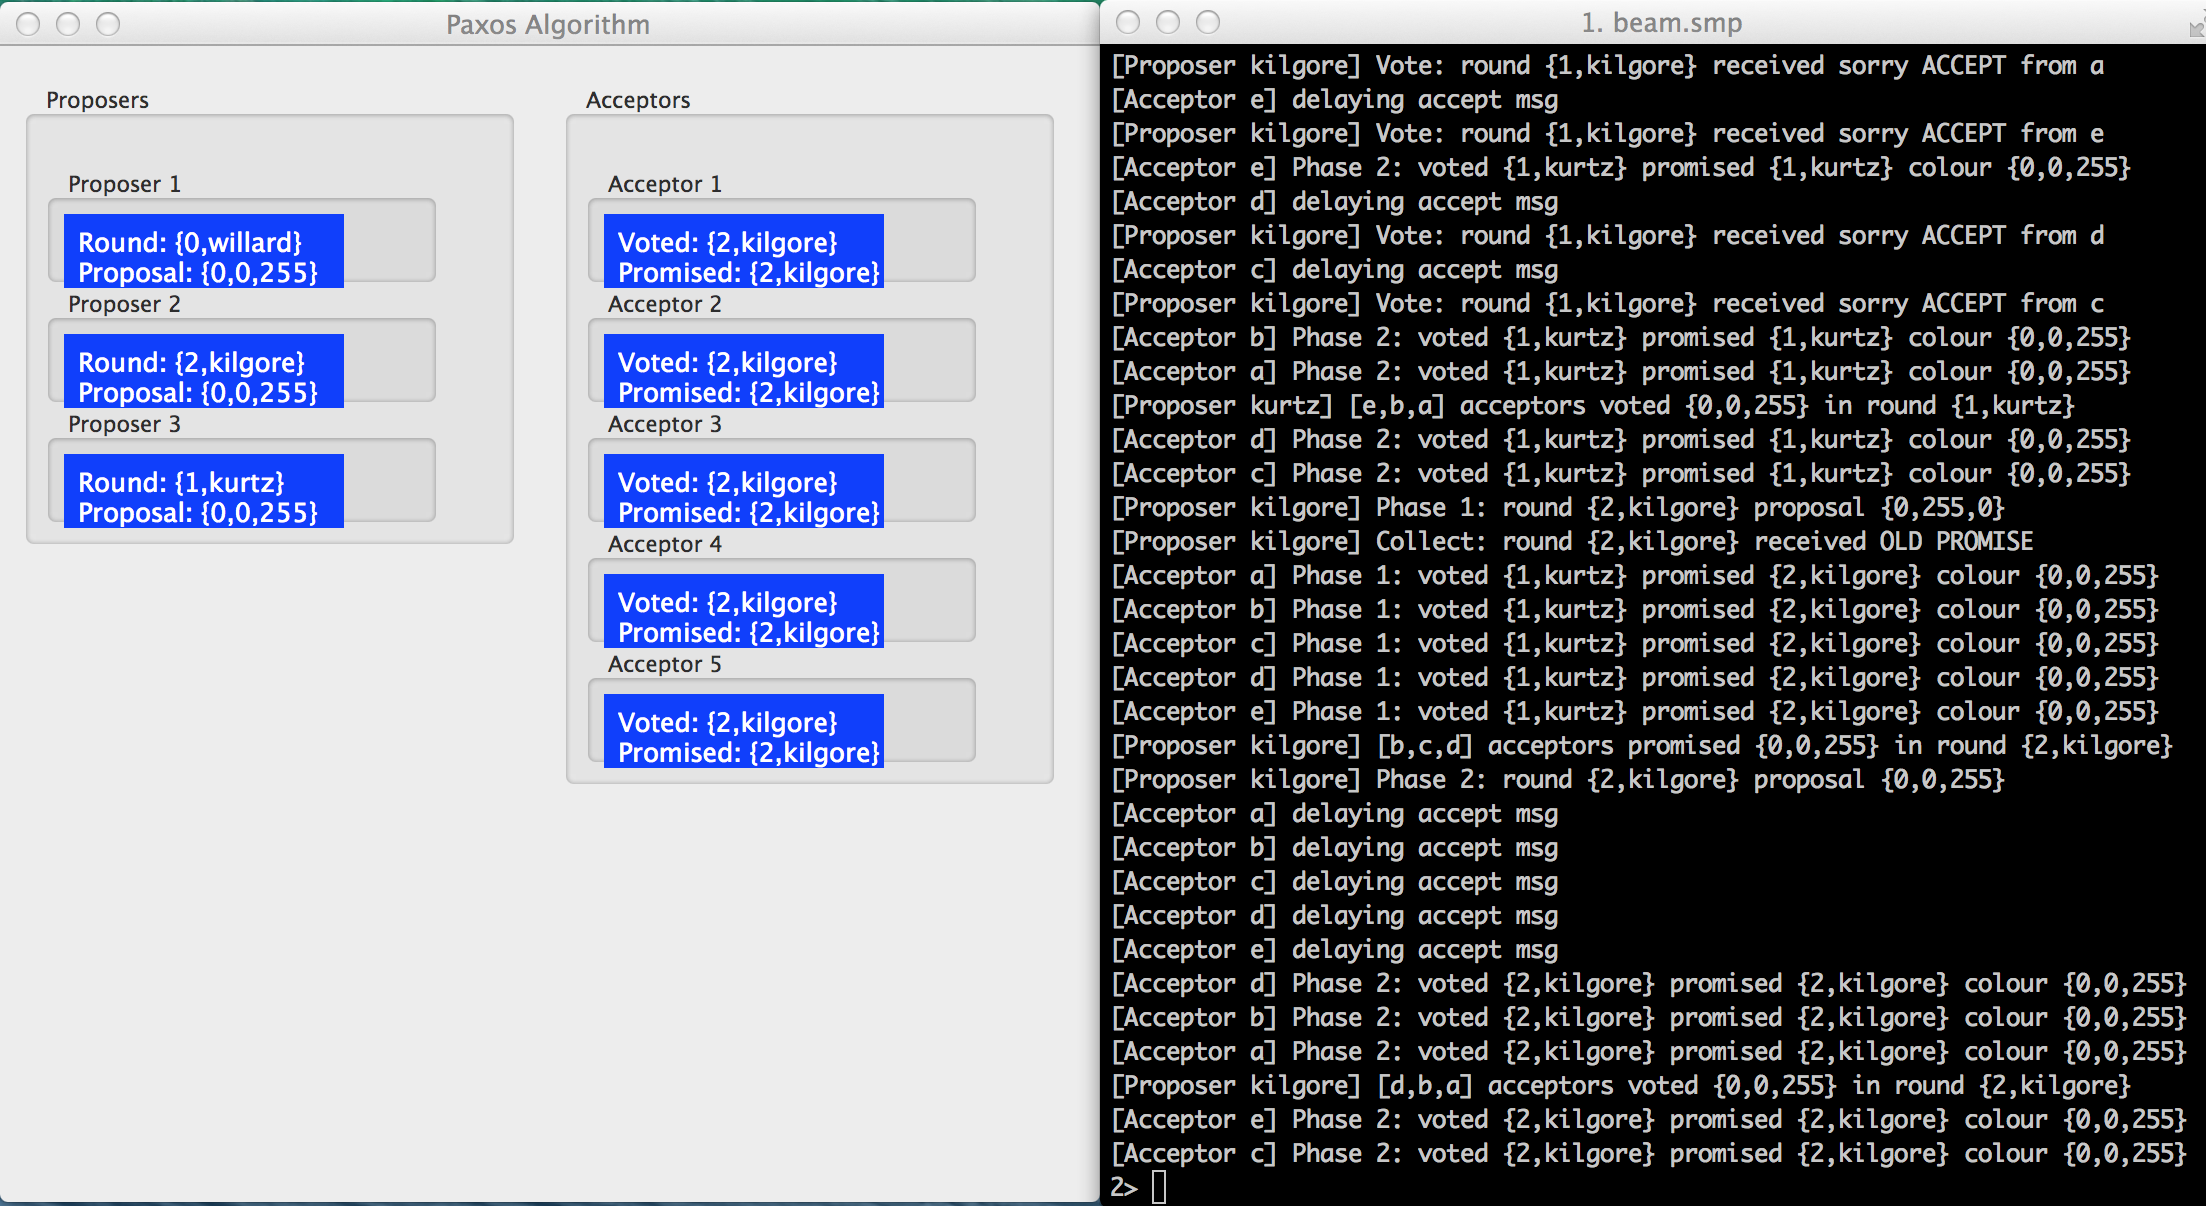
\includegraphics[scale=0.35]{images/exp2.png} \\\\
Lastly, we add delays both before \textit{prepare} and \textit{accept} messages are sent to proposers and the acceptors reach the same consensus again.\\

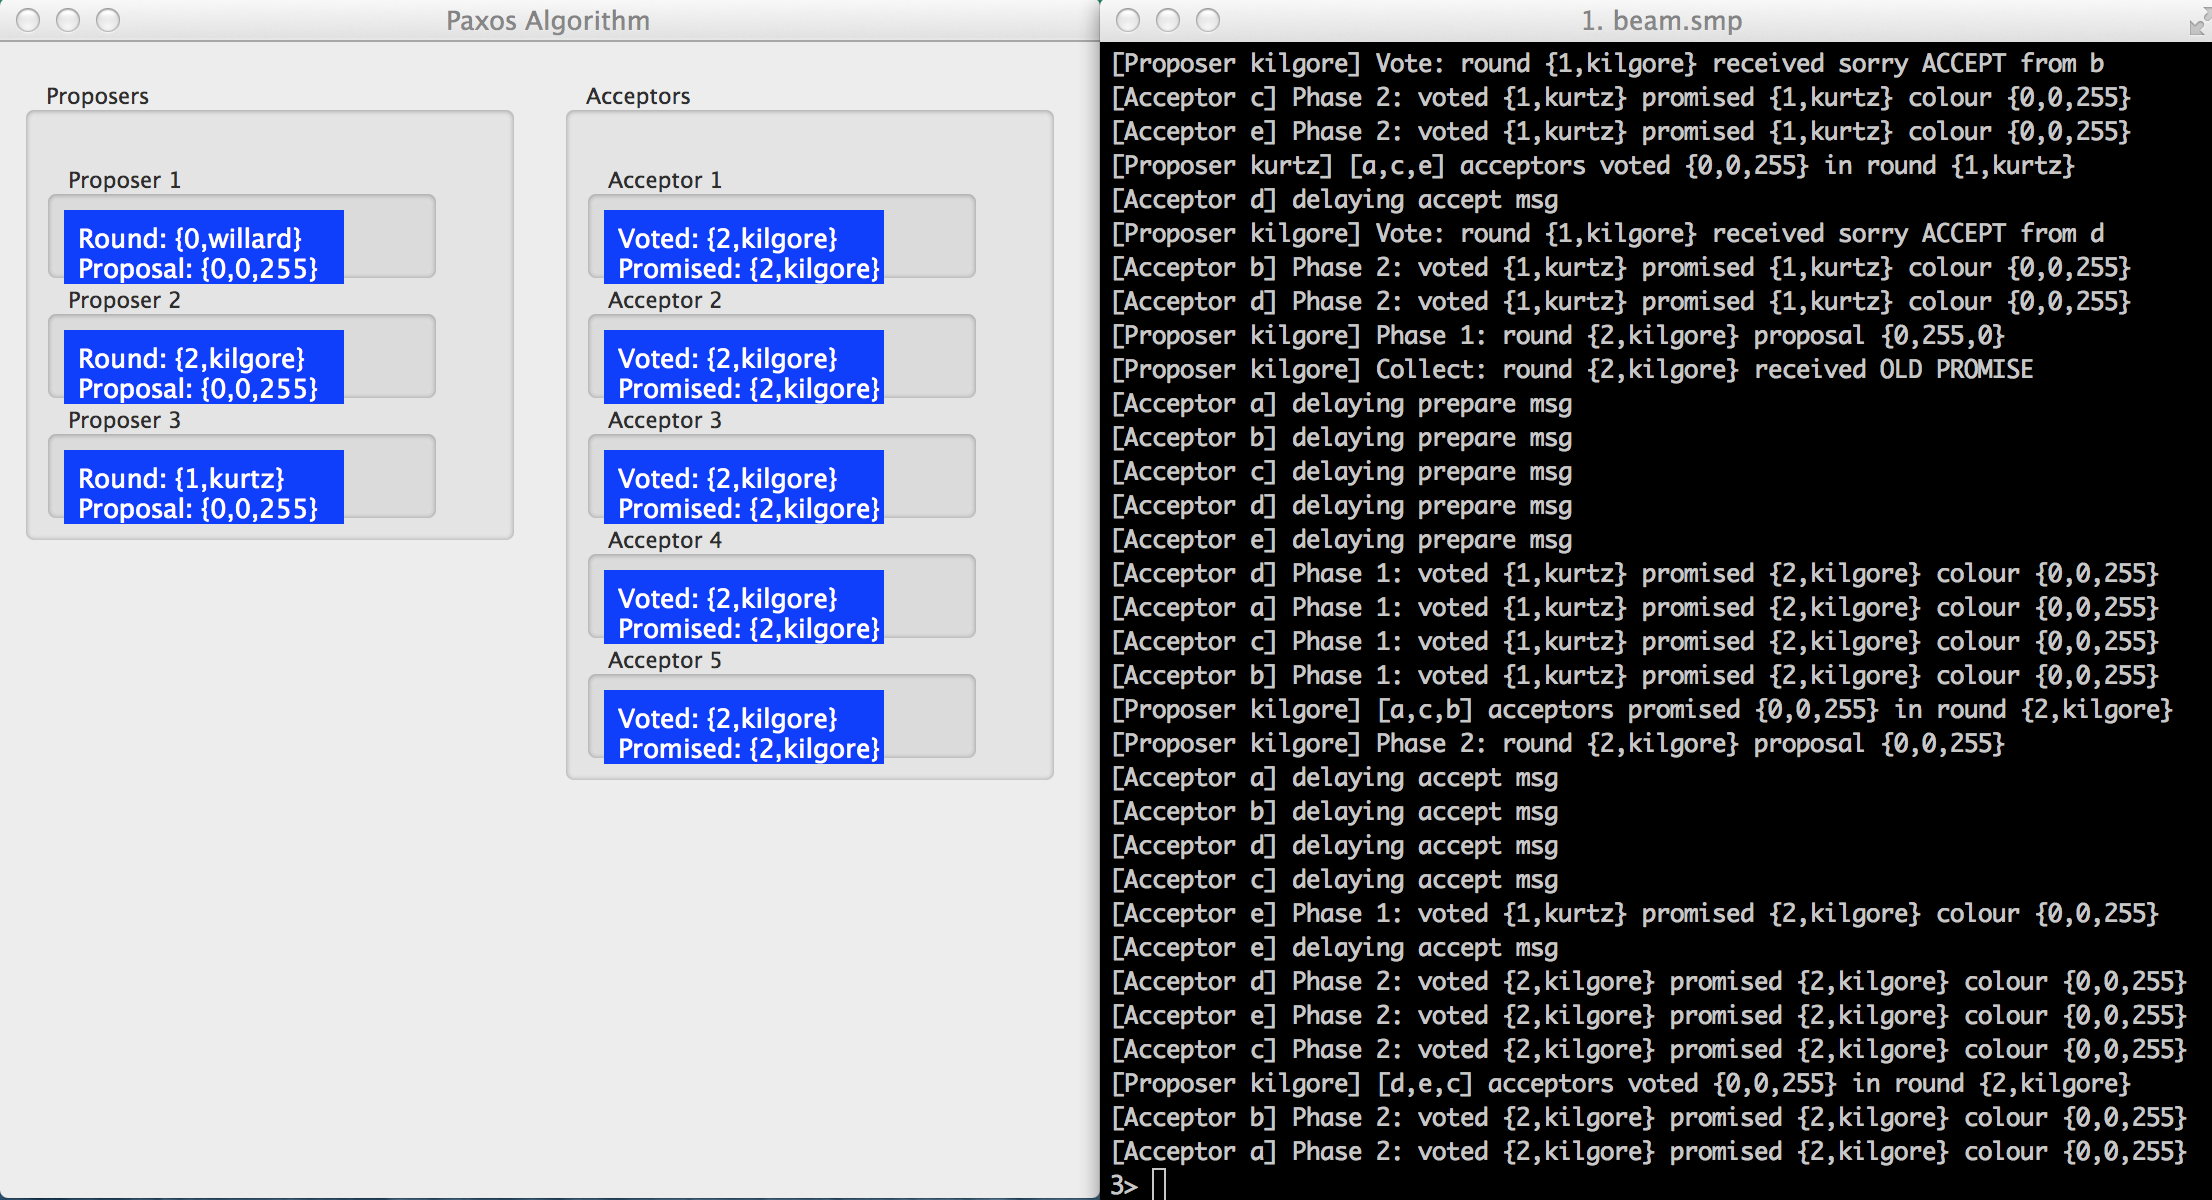
\includegraphics[scale=0.35]{images/exp3.png} \\\\
\newpage

\textbf{ii)} We stop sending \textit{sorry} messages to the processor and we run the experiment to try to reach a consensus.\\

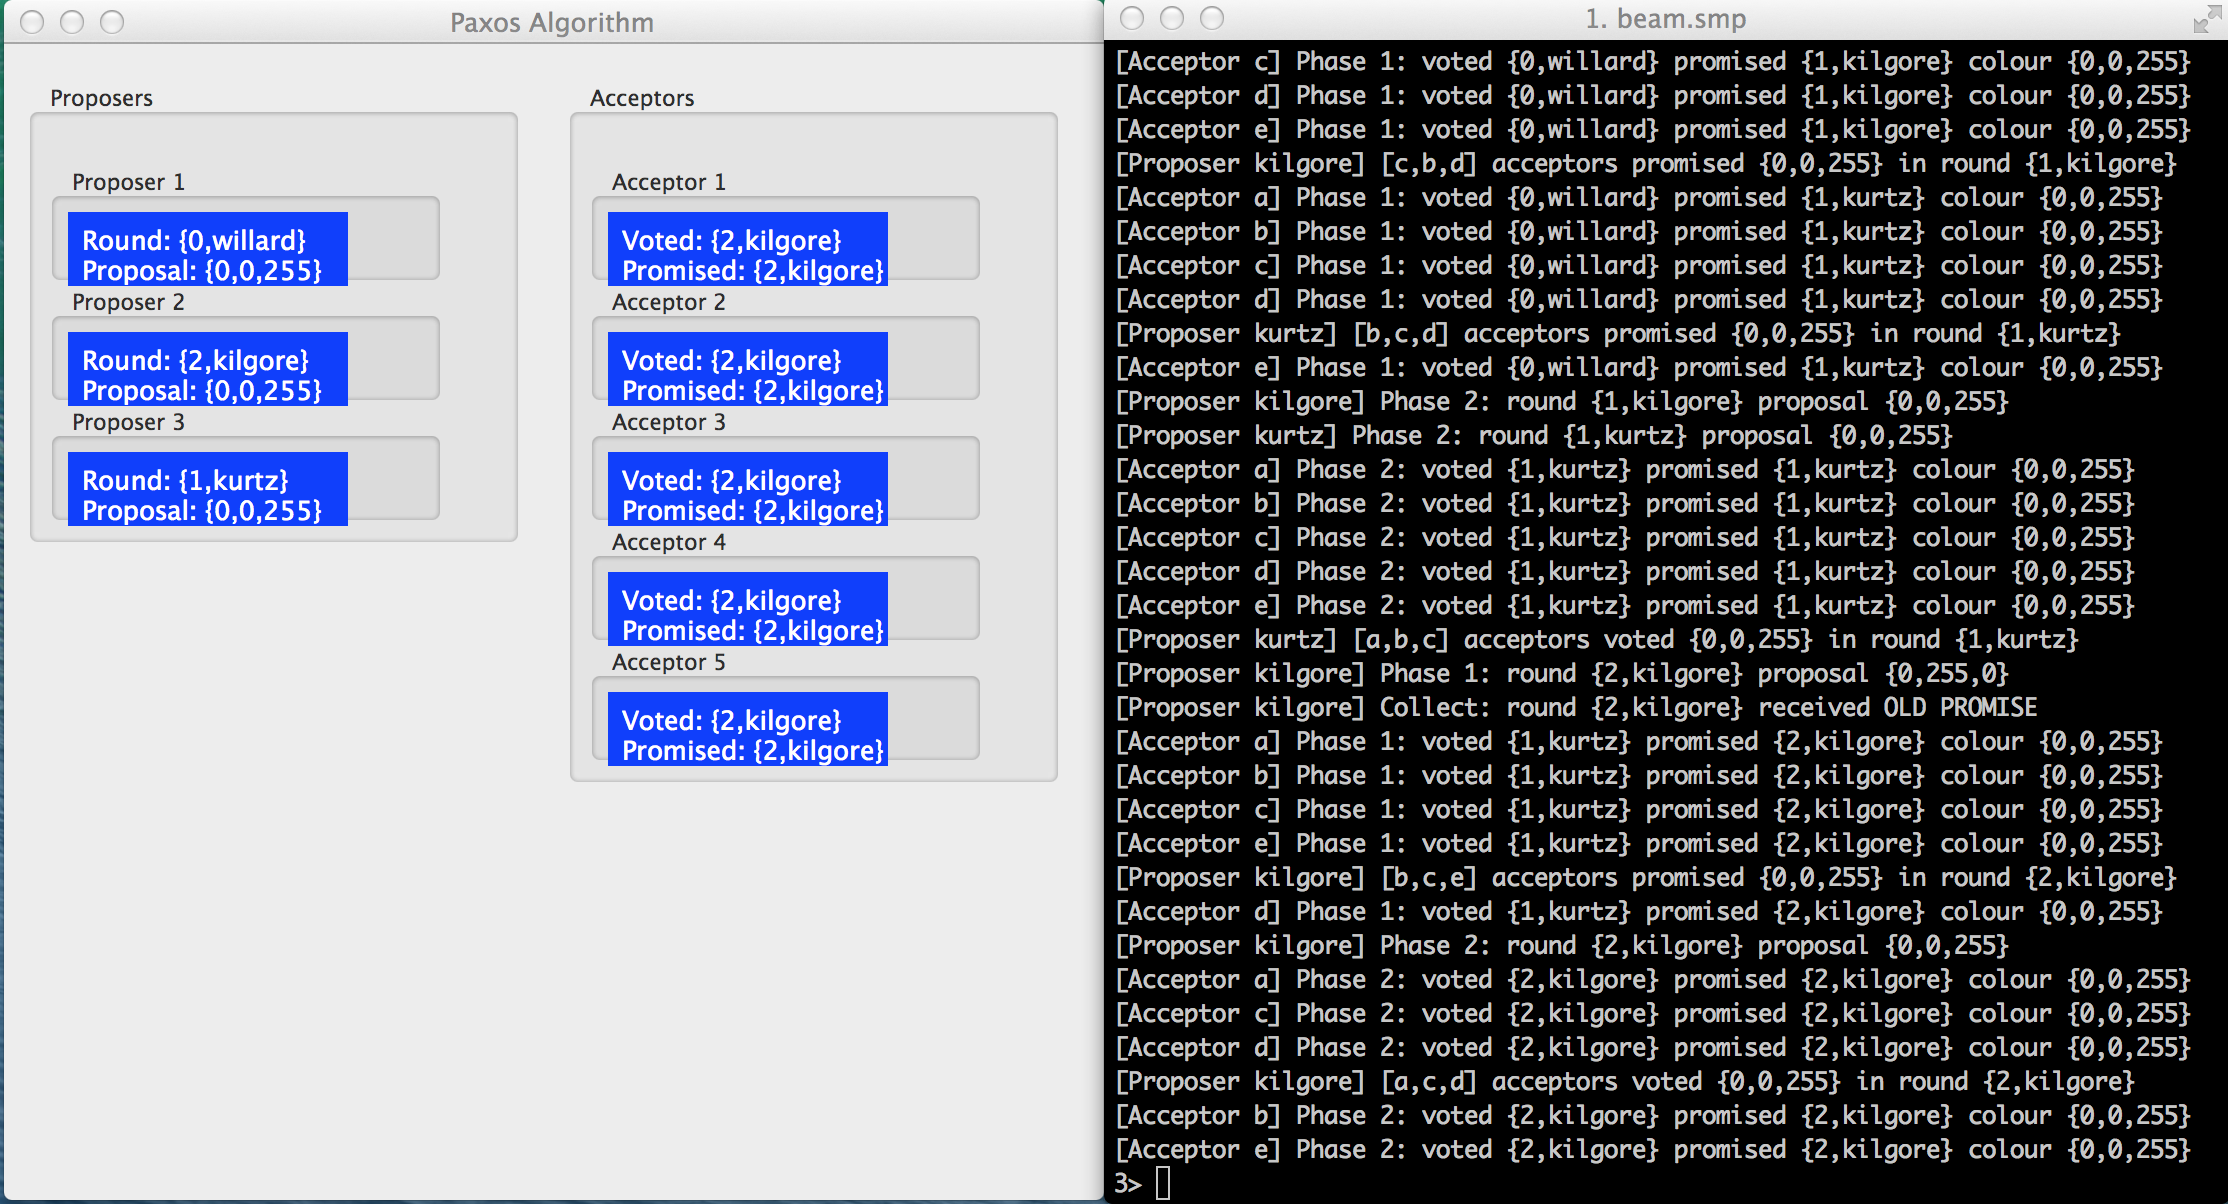
\includegraphics[scale=0.35]{images/exp4.png} \\\\

\textbf{iii)} In this experiment, we randomly drop \textit{promise} messages, and we look out for the consensus that the acceptors arrive to. Even though a promise message in round 2 is dropped, they still agree on the color blue.\\

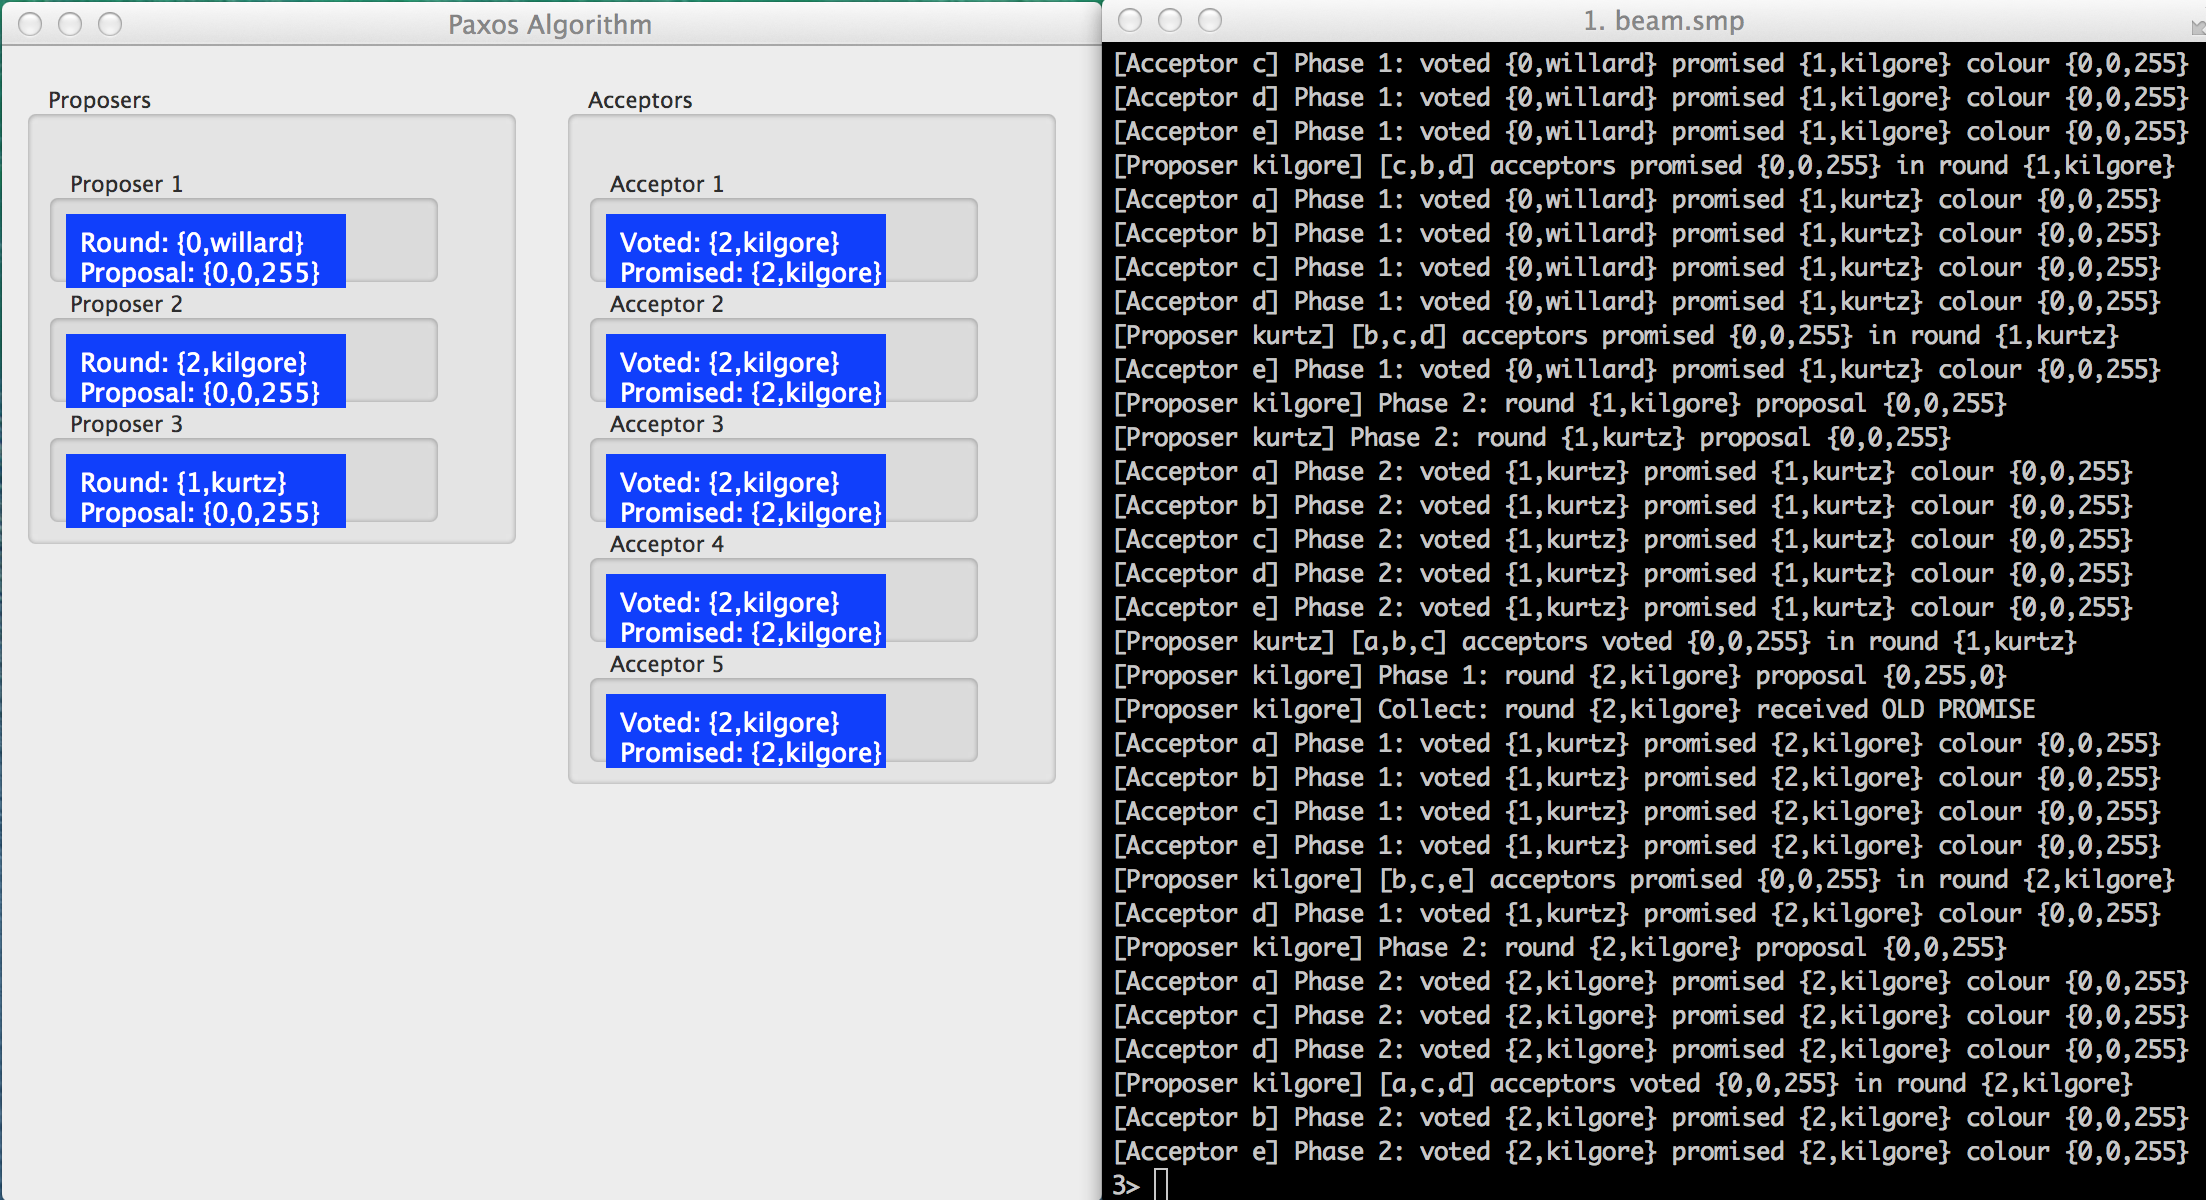
\includegraphics[scale=0.35]{images/exp5.png} \\\\
\newpage

Now, we run an experiment dropping \textit{vote} messages, this is, not replying to proposers with \textit{sorry} messages when asked to vote. Again, the acceptors manage to agree on the proposed color blue, even with a \textit{vote} message dropped because the other messages still amount to the majority of acceptors.\\

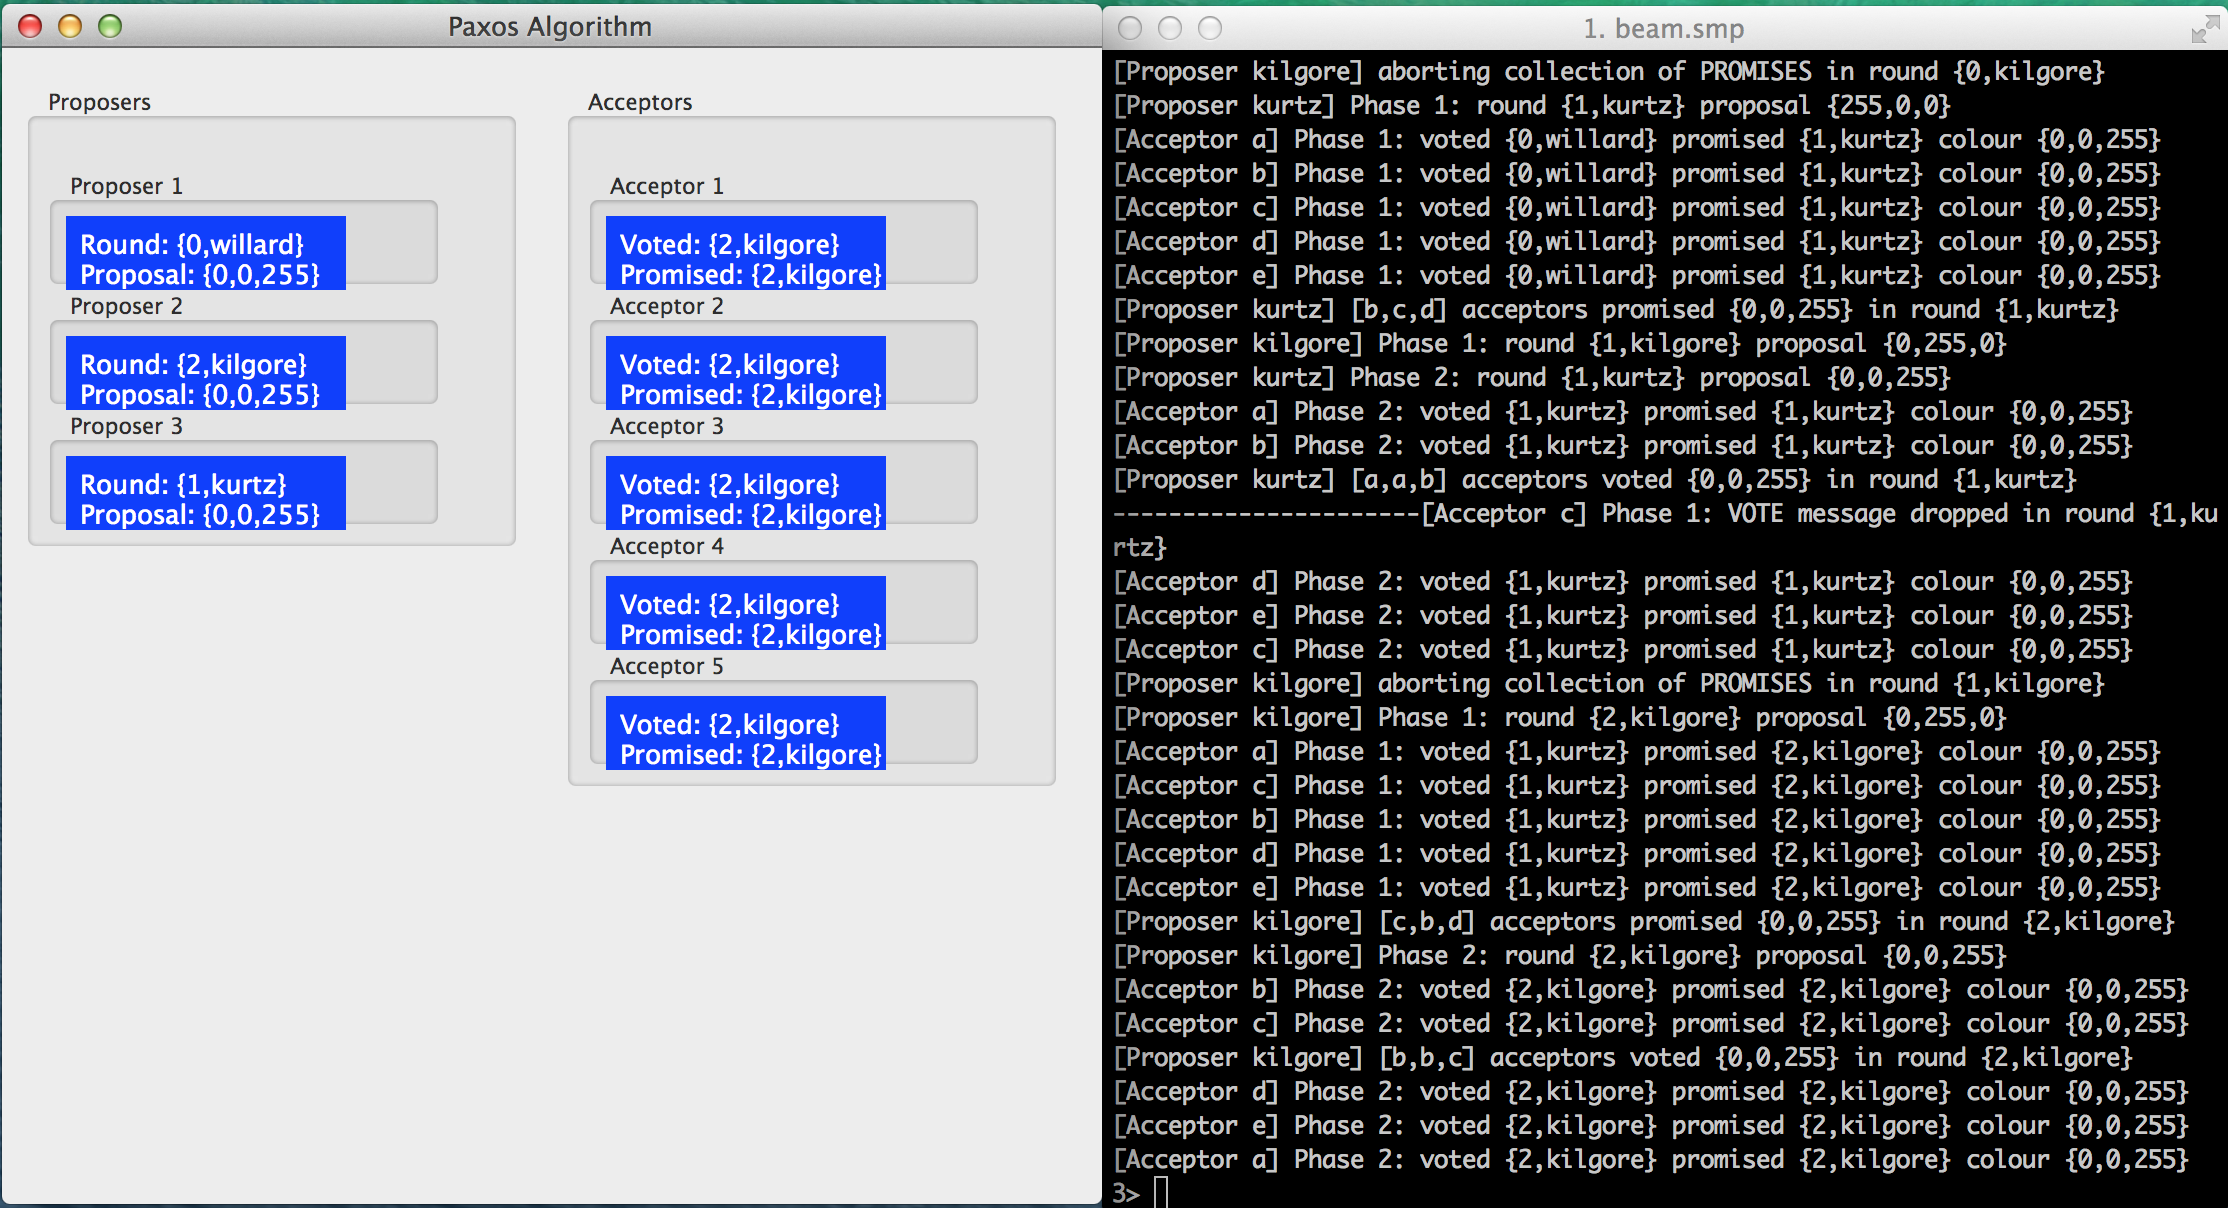
\includegraphics[scale=0.35]{images/exp6.png} \\\\

When we run the experiment dropping both \textit{promise} and \textit{vote} \textit{sorry} messages, we see that the algorithm still terminates successfully due to the fact that the majority of acceptors whose messages were not dropped agreed.\\

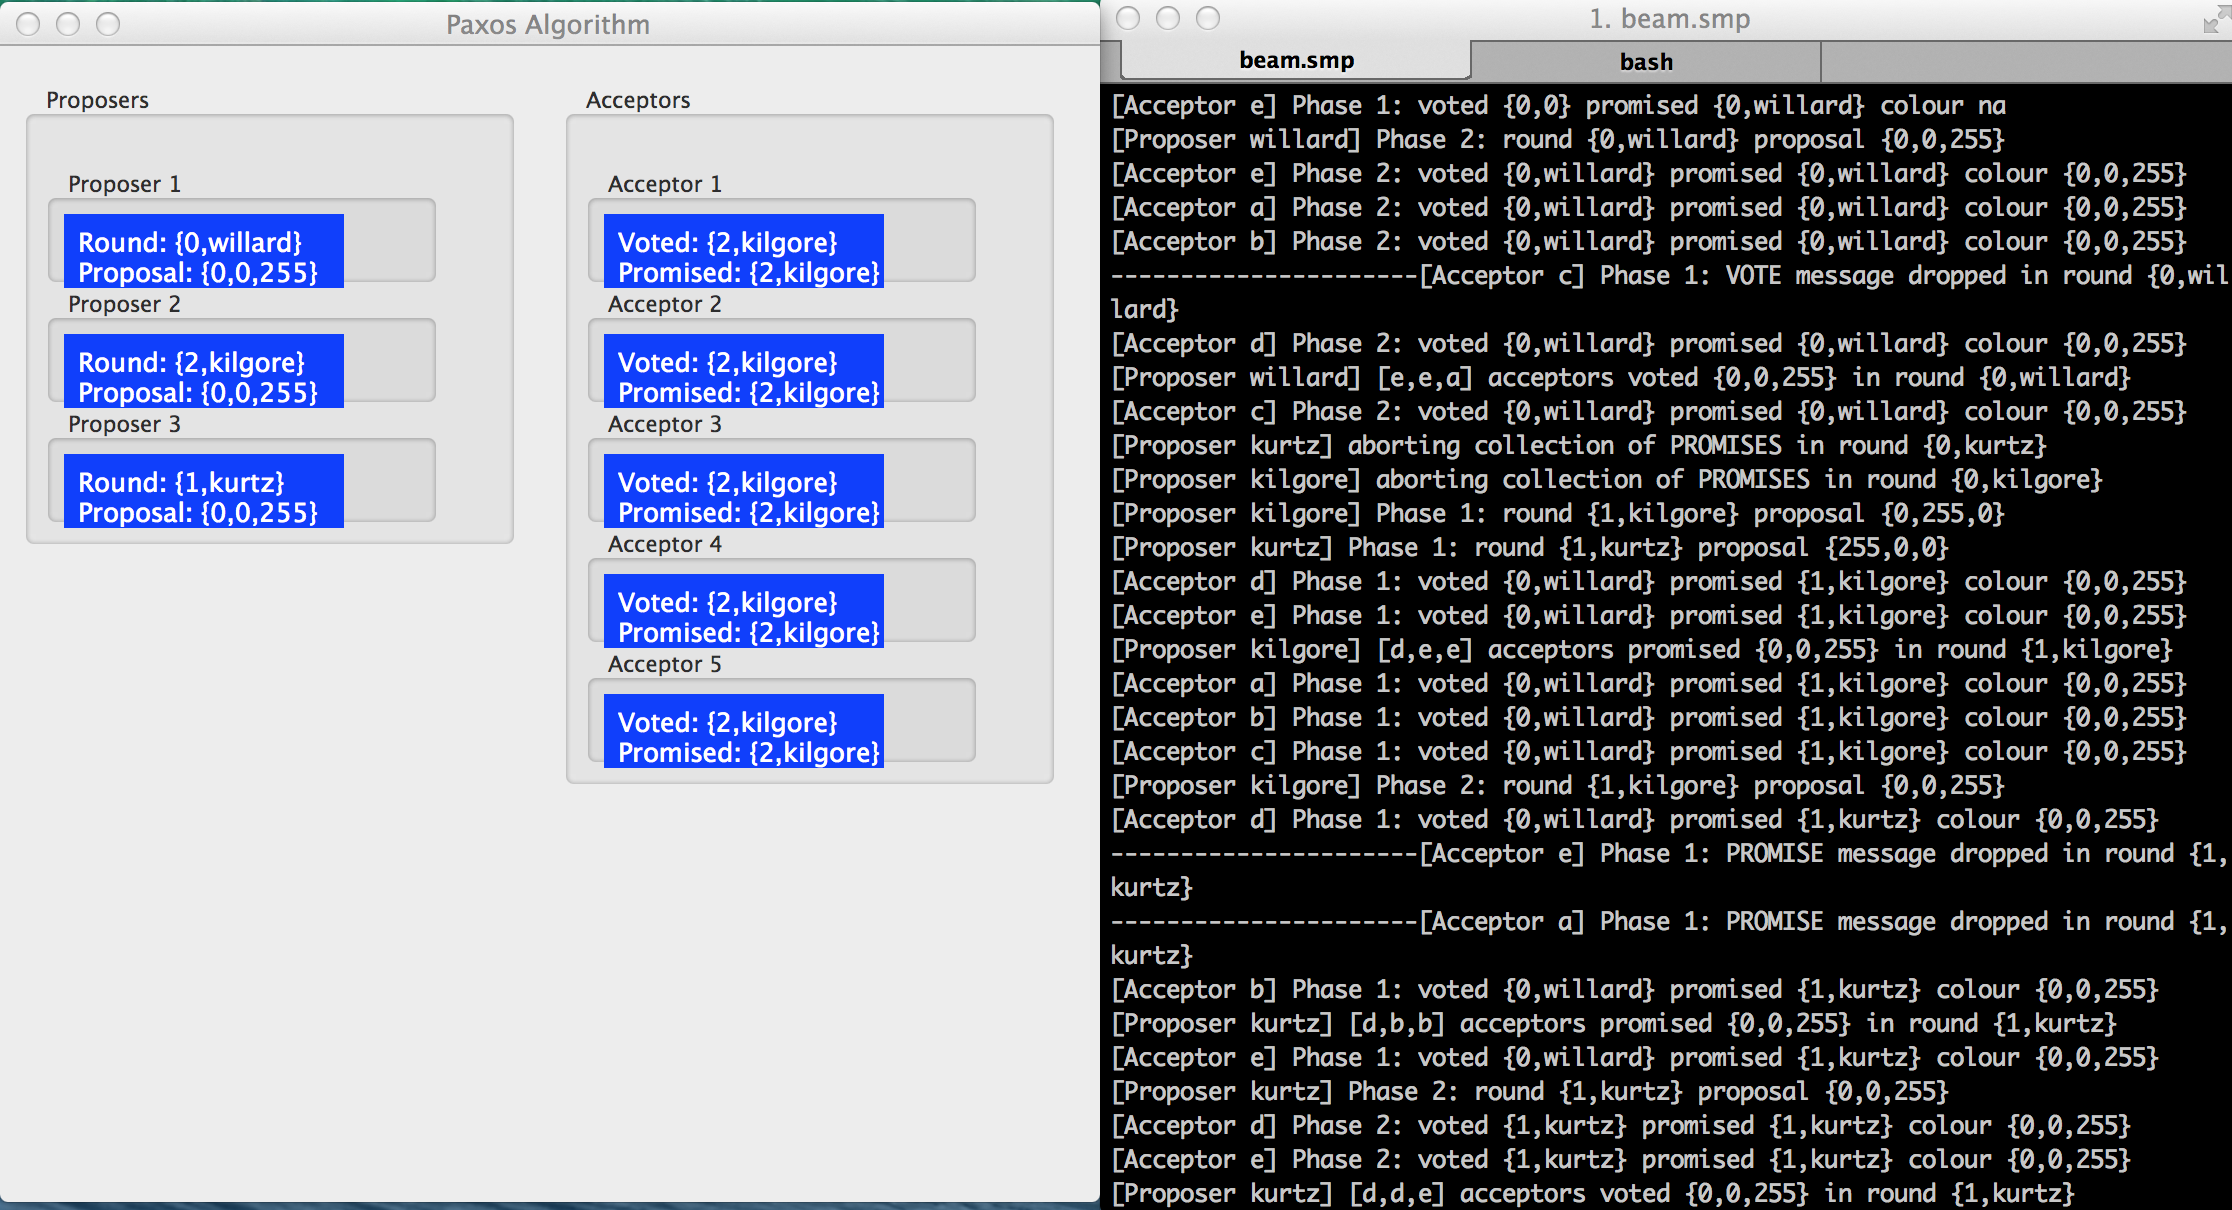
\includegraphics[scale=0.35]{images/exp7.png} \\\\

We also run the experiment by dropping more than one \textit{promise} and \textit{vote} messages in a total of 10 messages. Here is the result of dropping one message in 5. The algorithm still terminates and the acceptors reach the consensus.\\

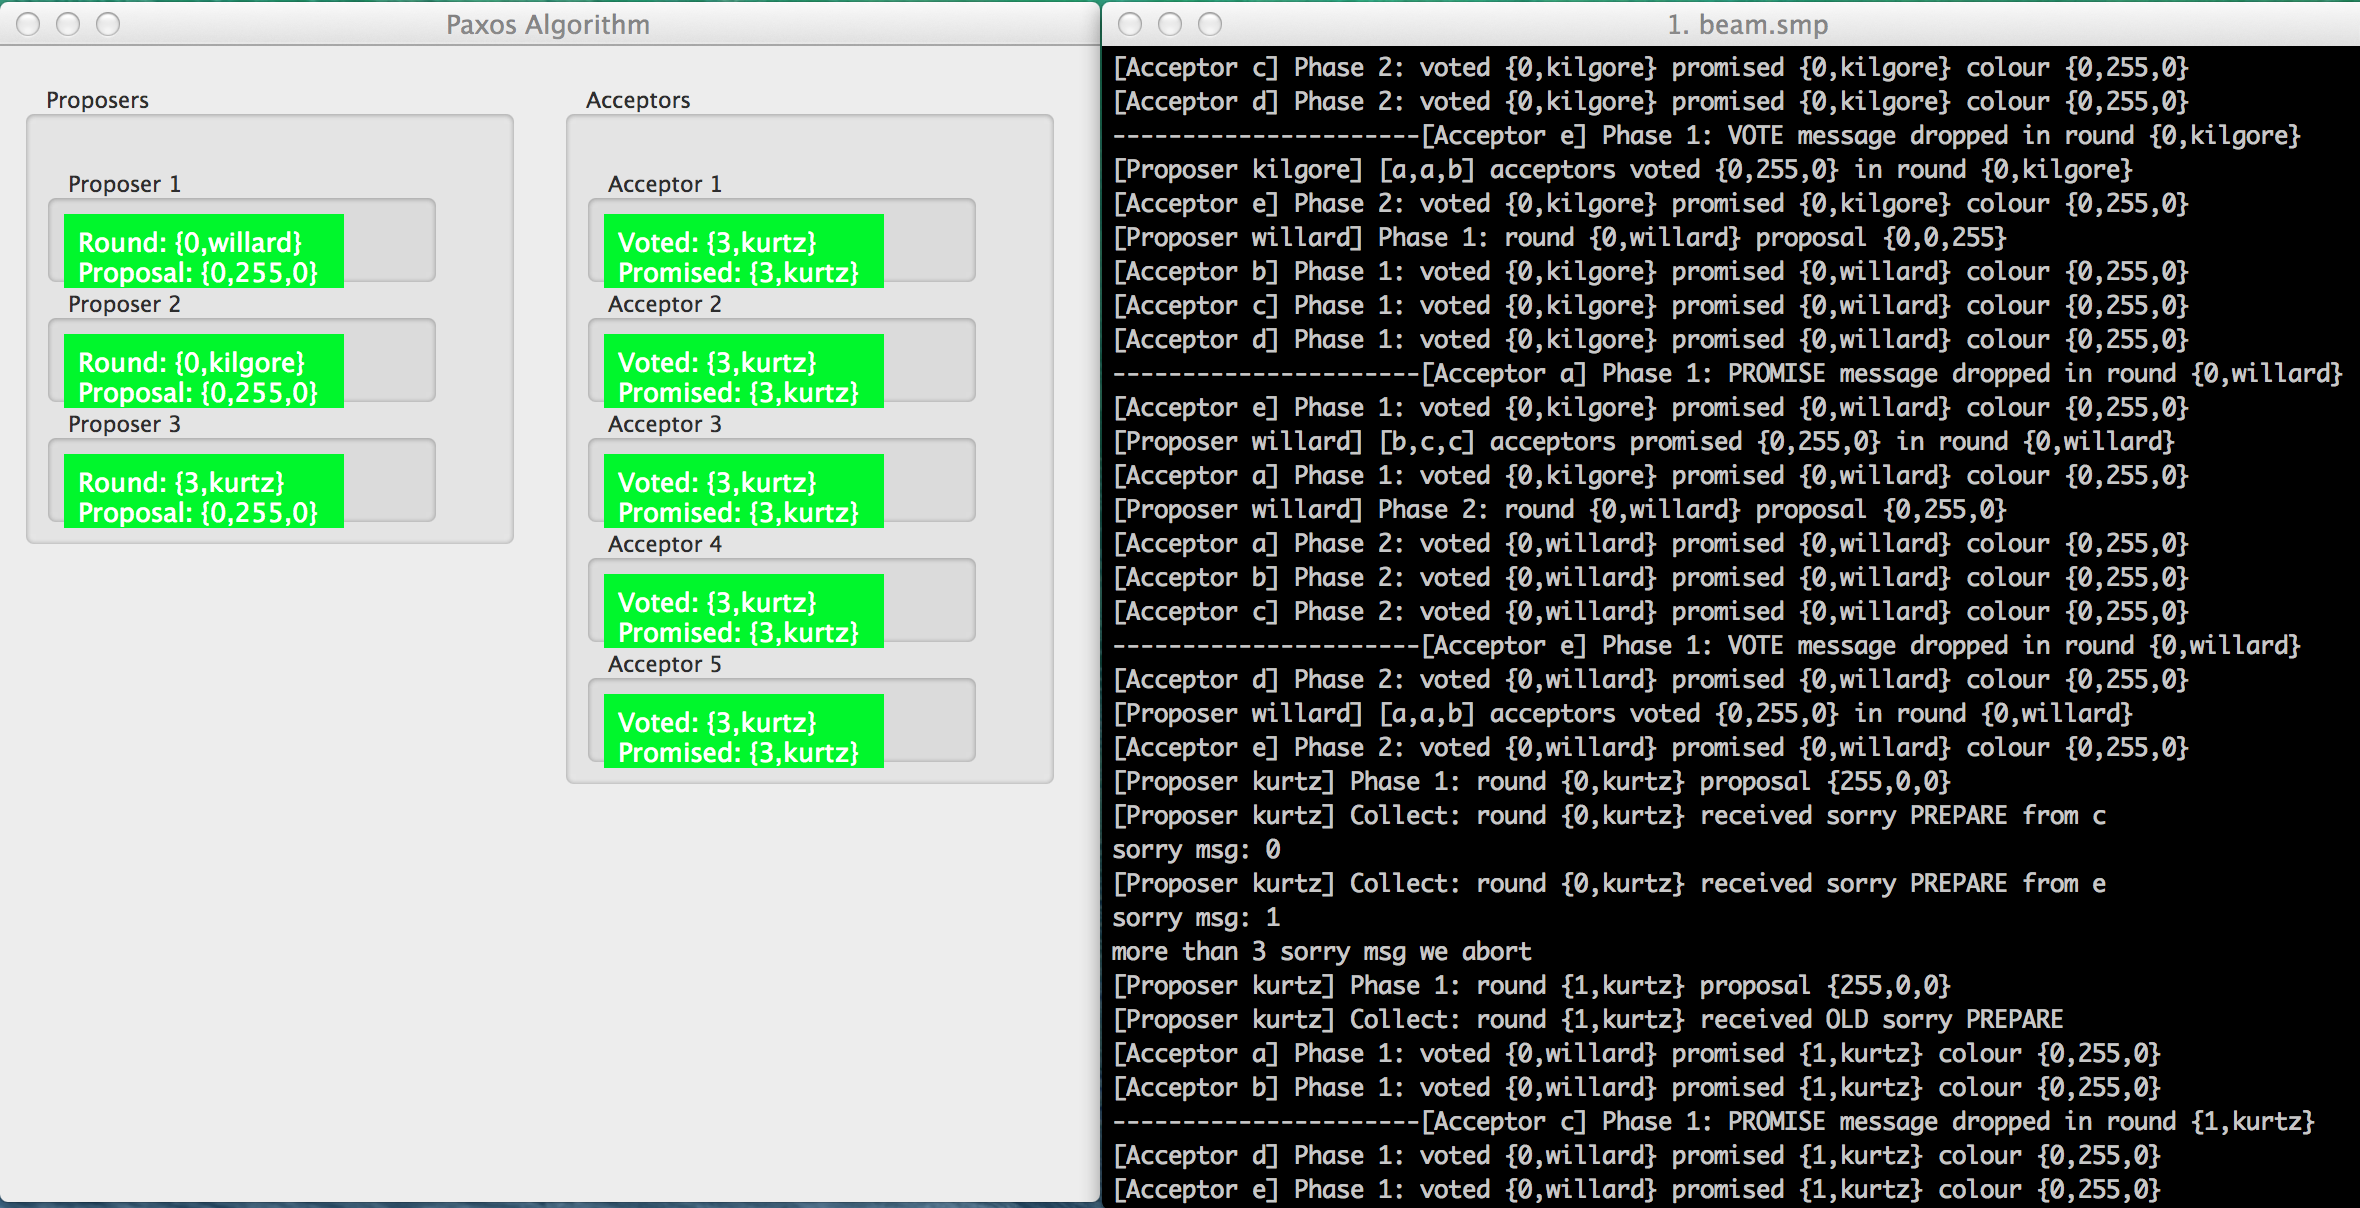
\includegraphics[scale=0.35]{images/exp7-drop5.png} \\\\

We ran more experiments by dropping one message in 3:\\

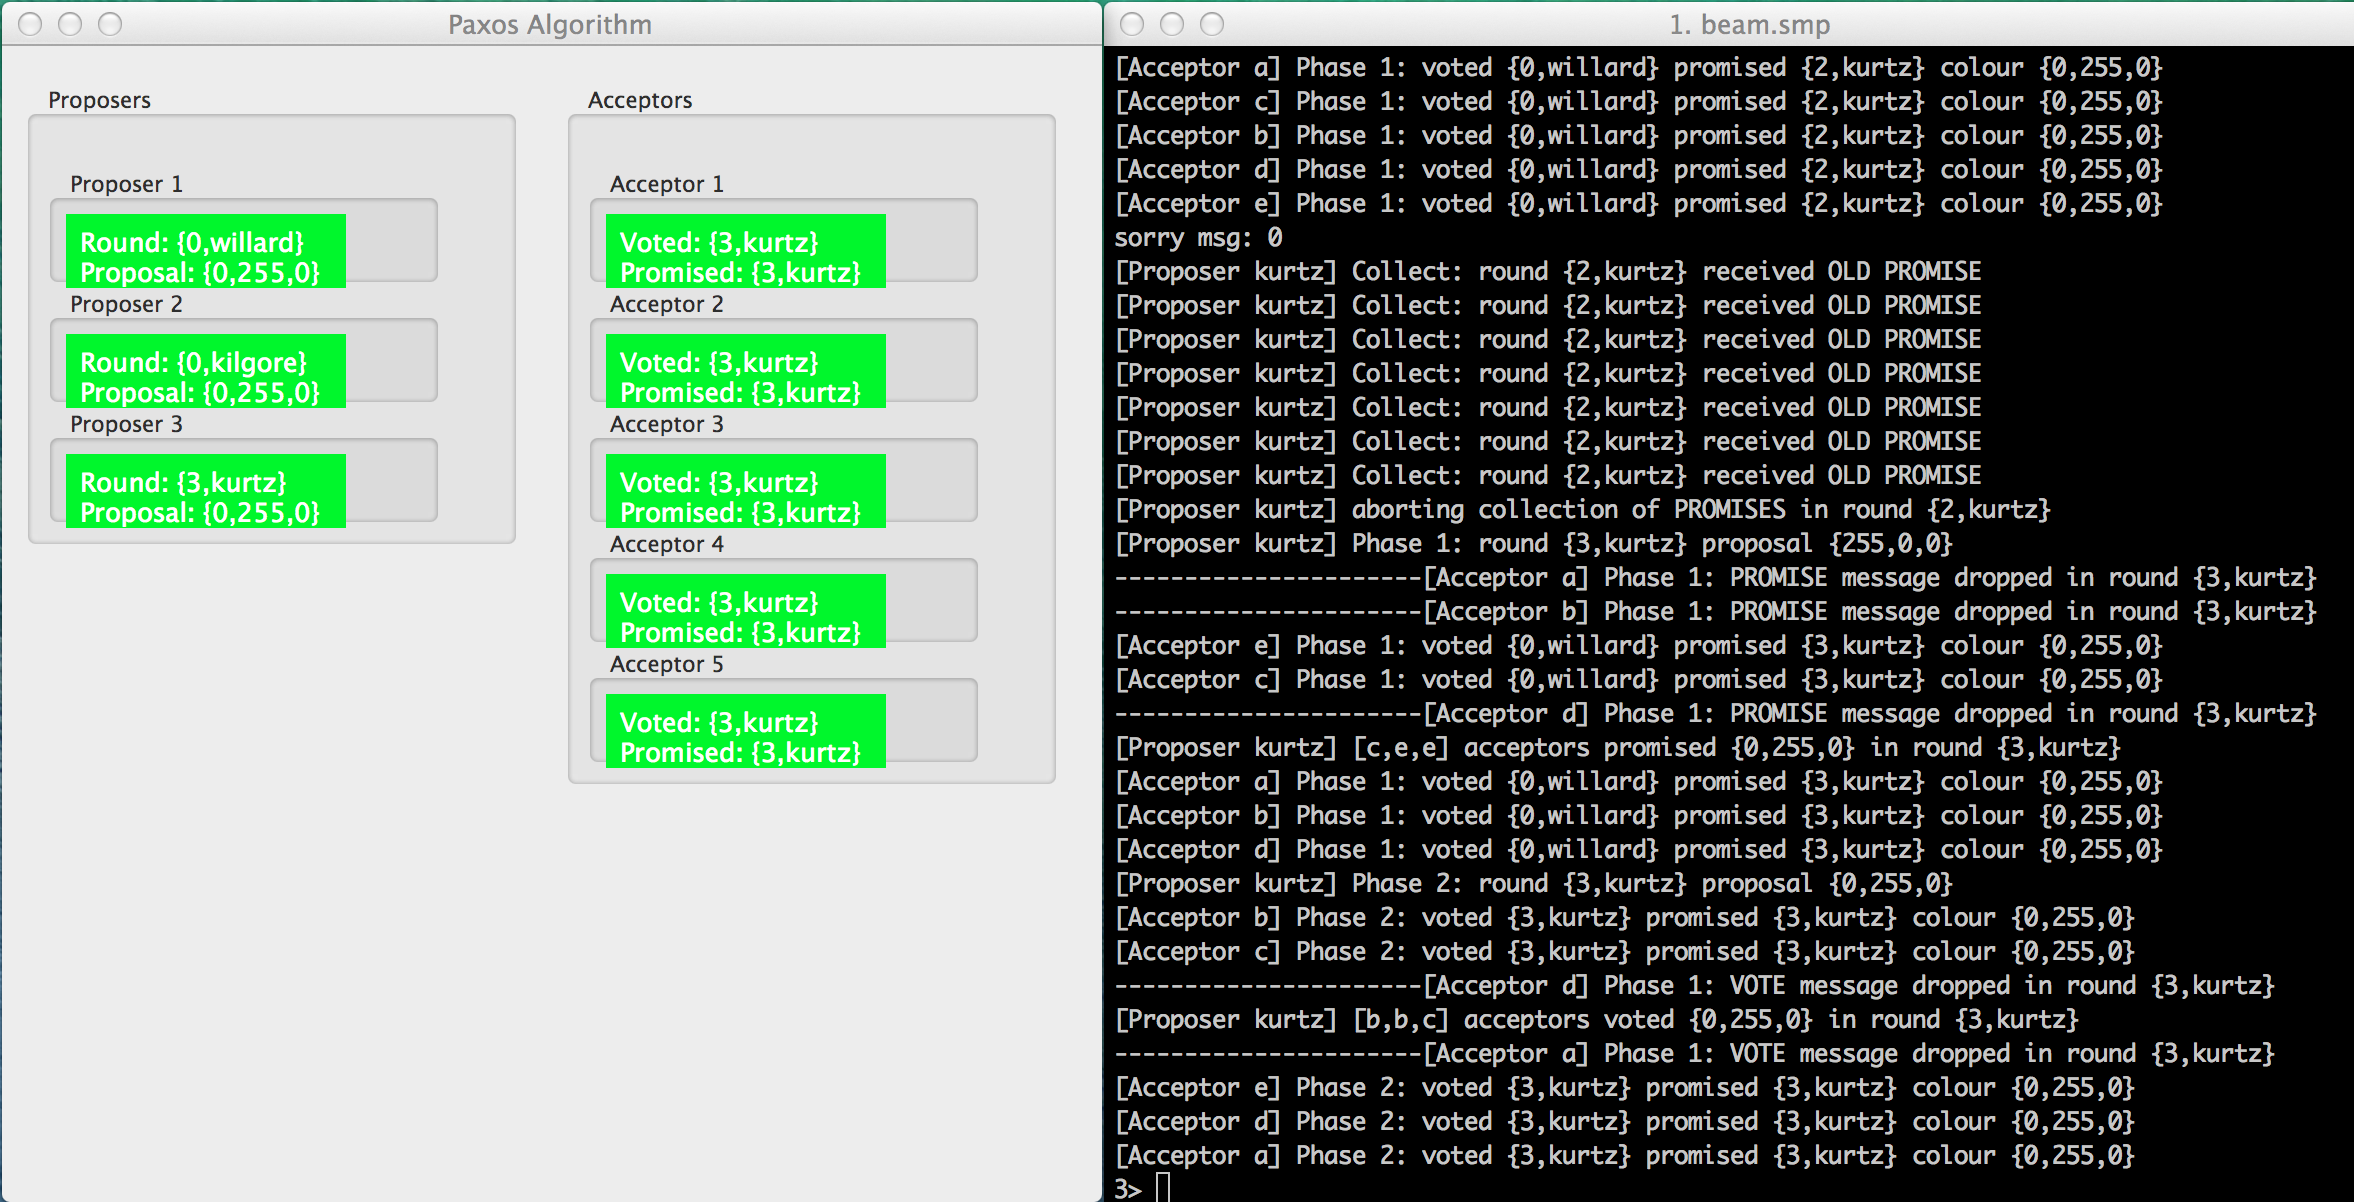
\includegraphics[scale=0.35]{images/exp7-drop3.png} \\\\
\newpage

And one message in 1:\\

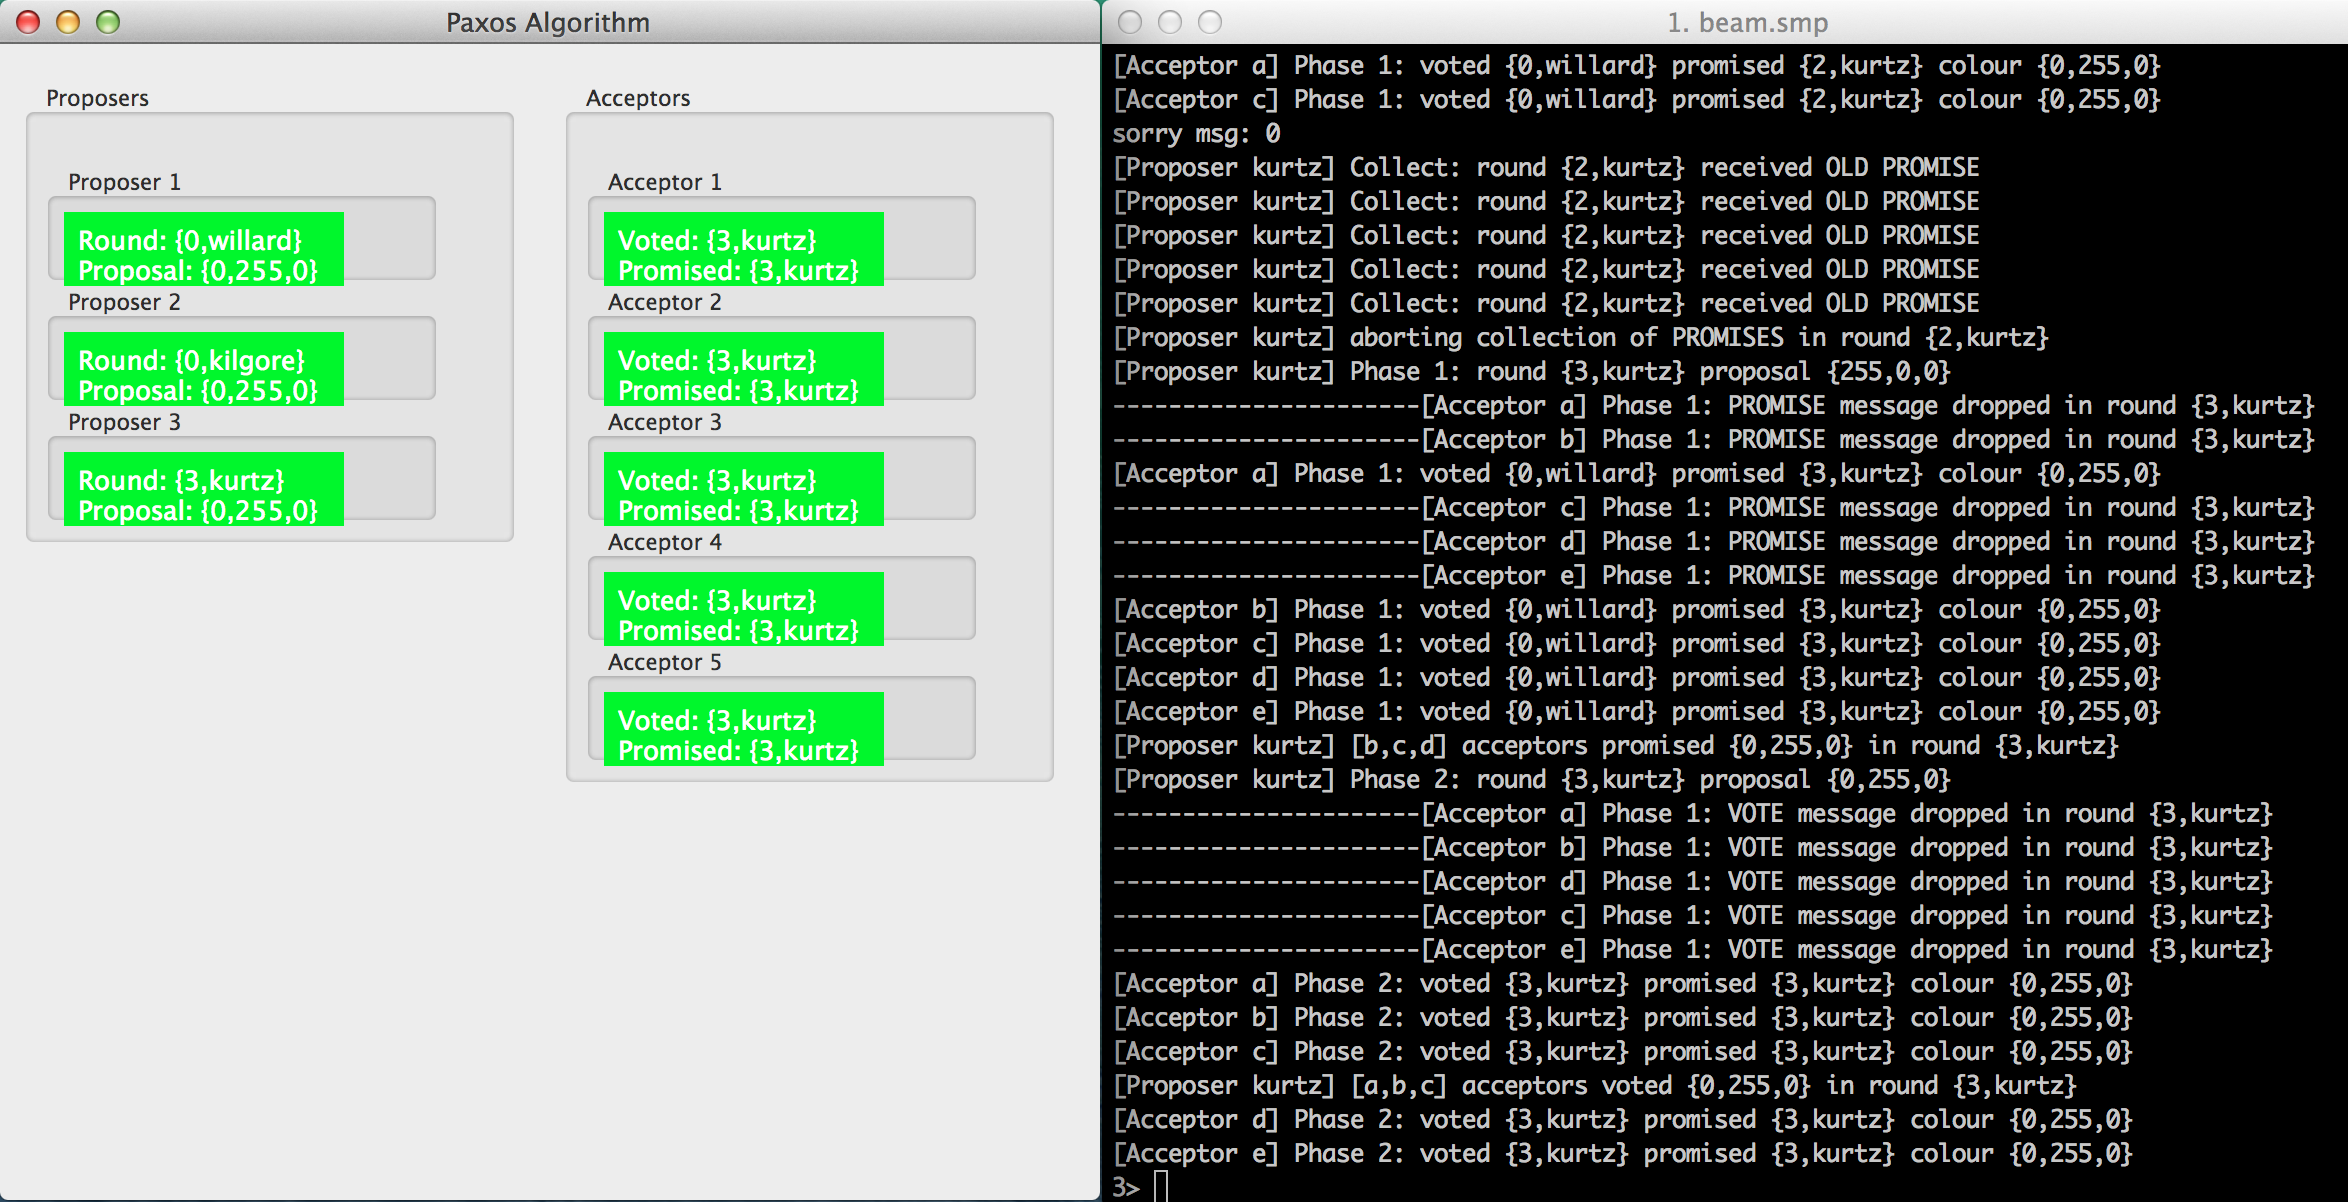
\includegraphics[scale=0.35]{images/exp7-drop1.png} \\\\

And even though more and more messages are dropped an agreement is eventually met. However if we add the line: \textit{-define(drop, 0).} then the algorithm does not terminate.\\

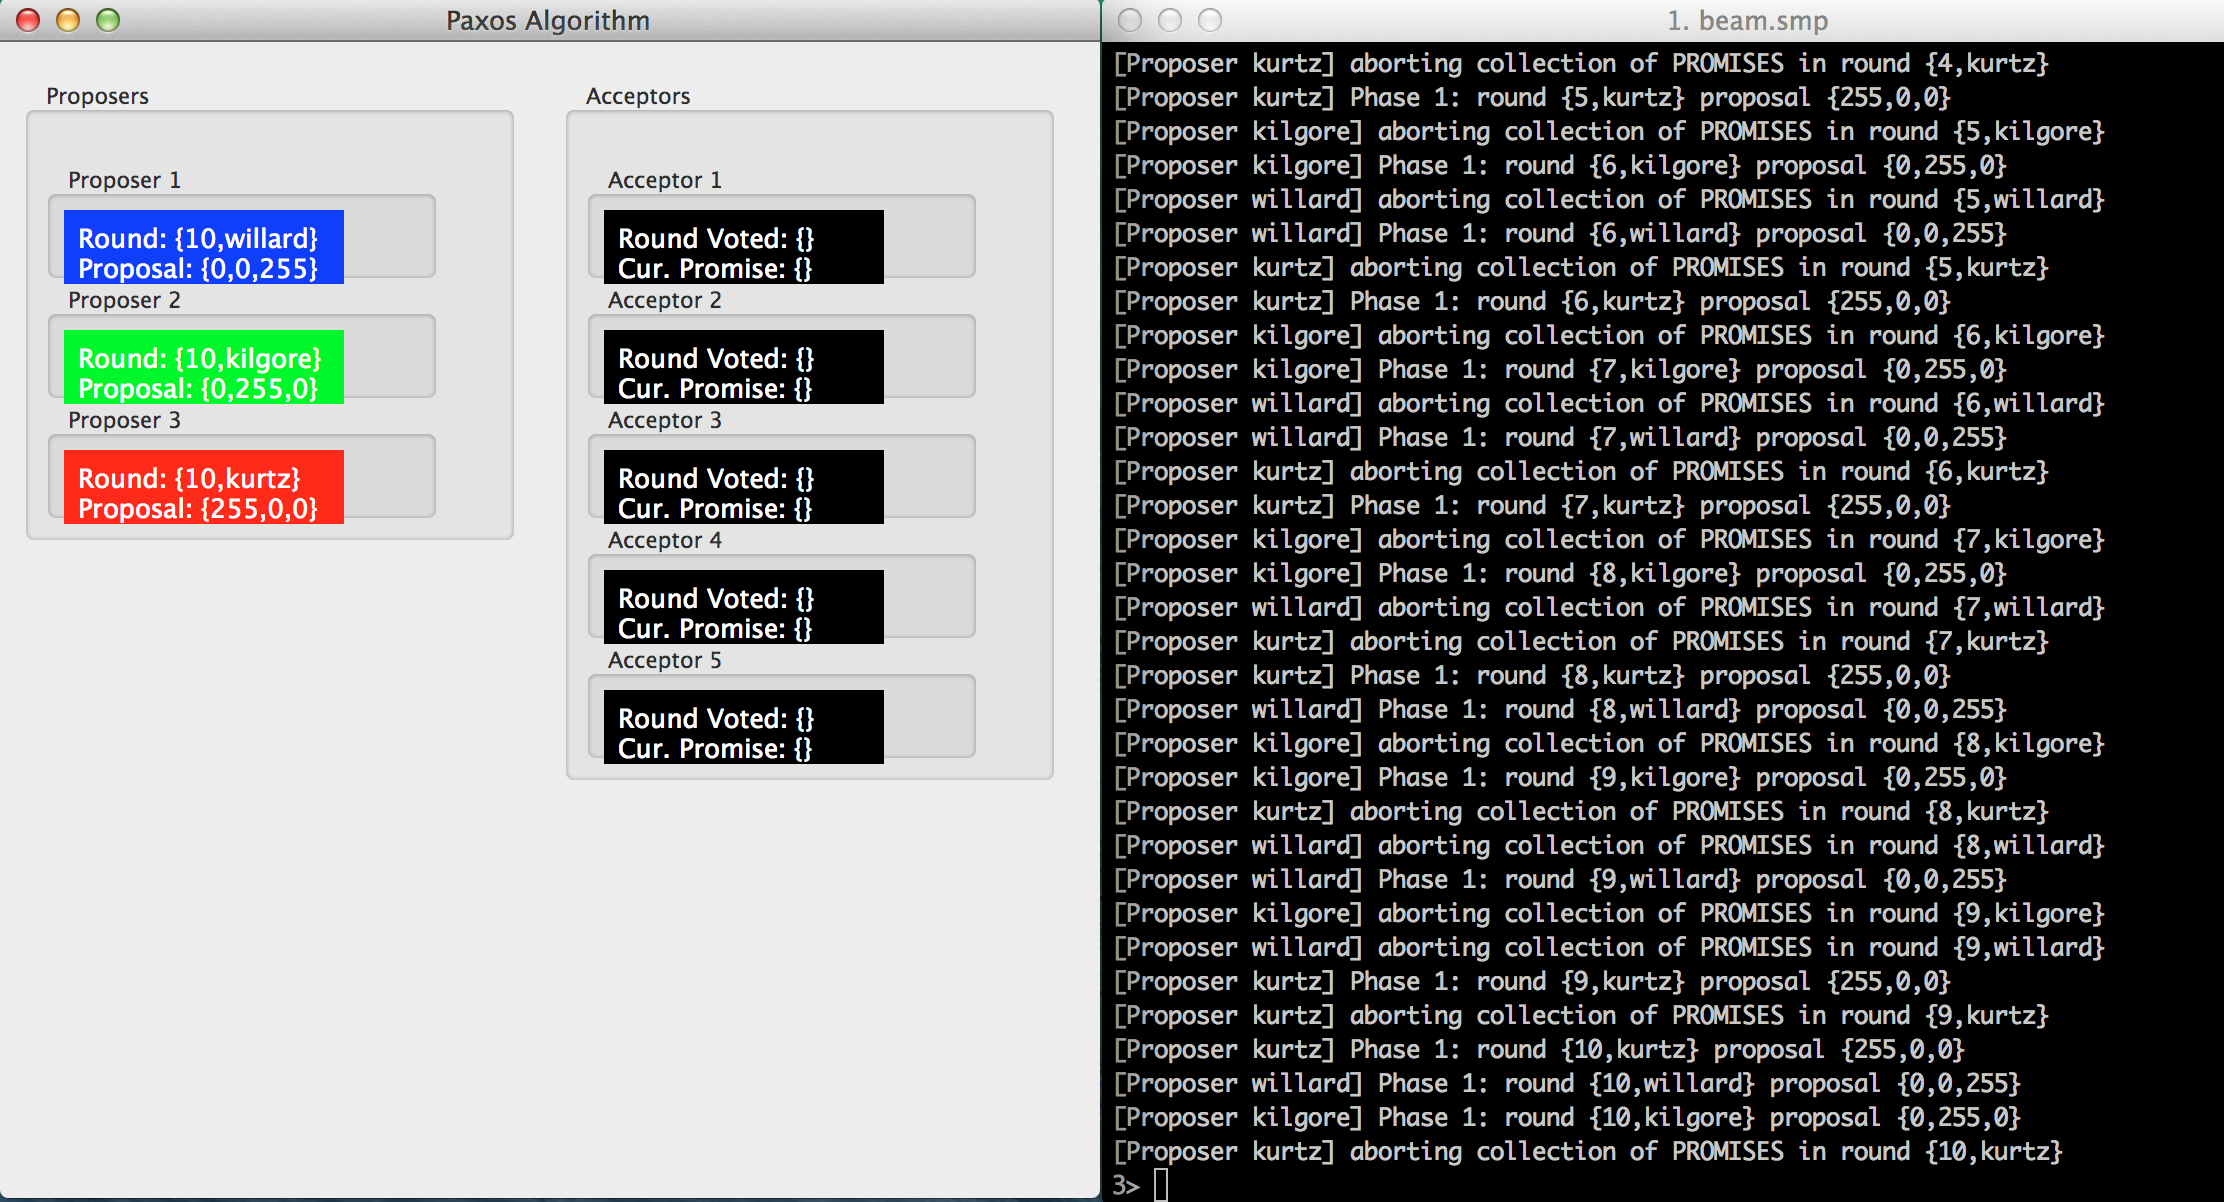
\includegraphics[scale=0.35]{images/exp7-drop0.png} \\\\
\newpage

\textbf{iv)} We increase the number of acceptors to 10 and the number or proposers to 6. The acceptors still get to a consensuns in round 3 on color \textit{purple}.\\

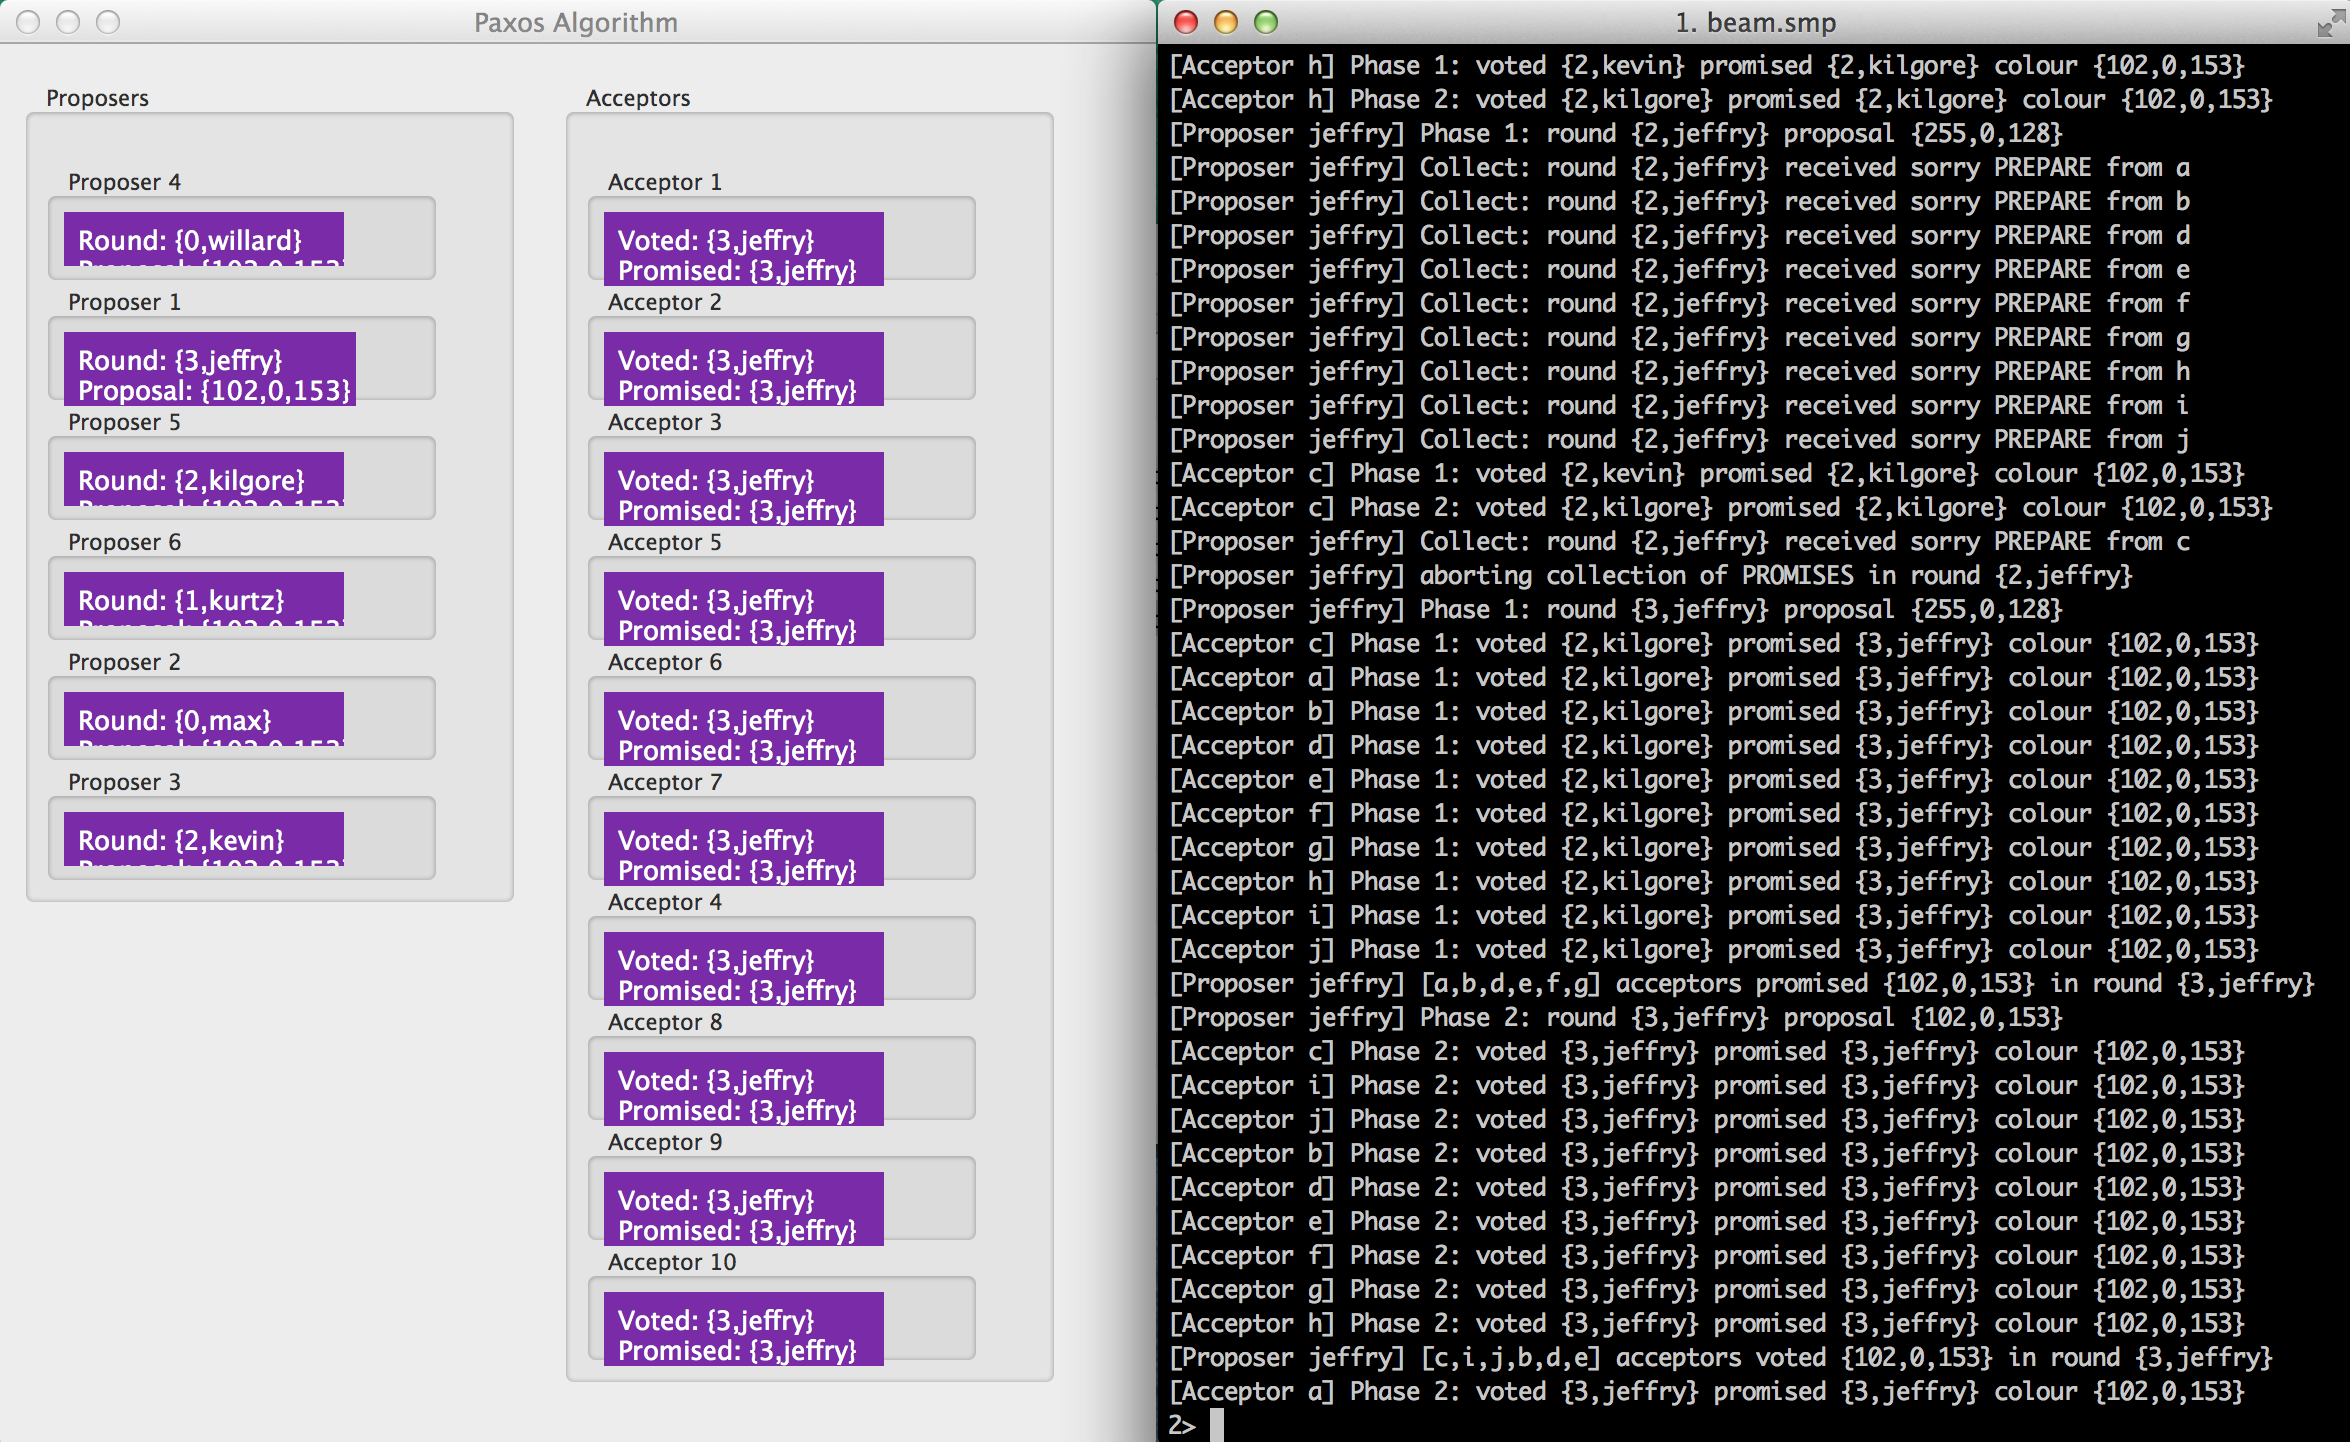
\includegraphics[scale=0.30]{images/exp8.png} \\\\

\textbf{v)} In this experiment we changed the modules to adjust them such that we can run the proposers in one node and the acceptors in a different one and as they communicate they reach an agreement on the color \textit{blue} in round 2.\\

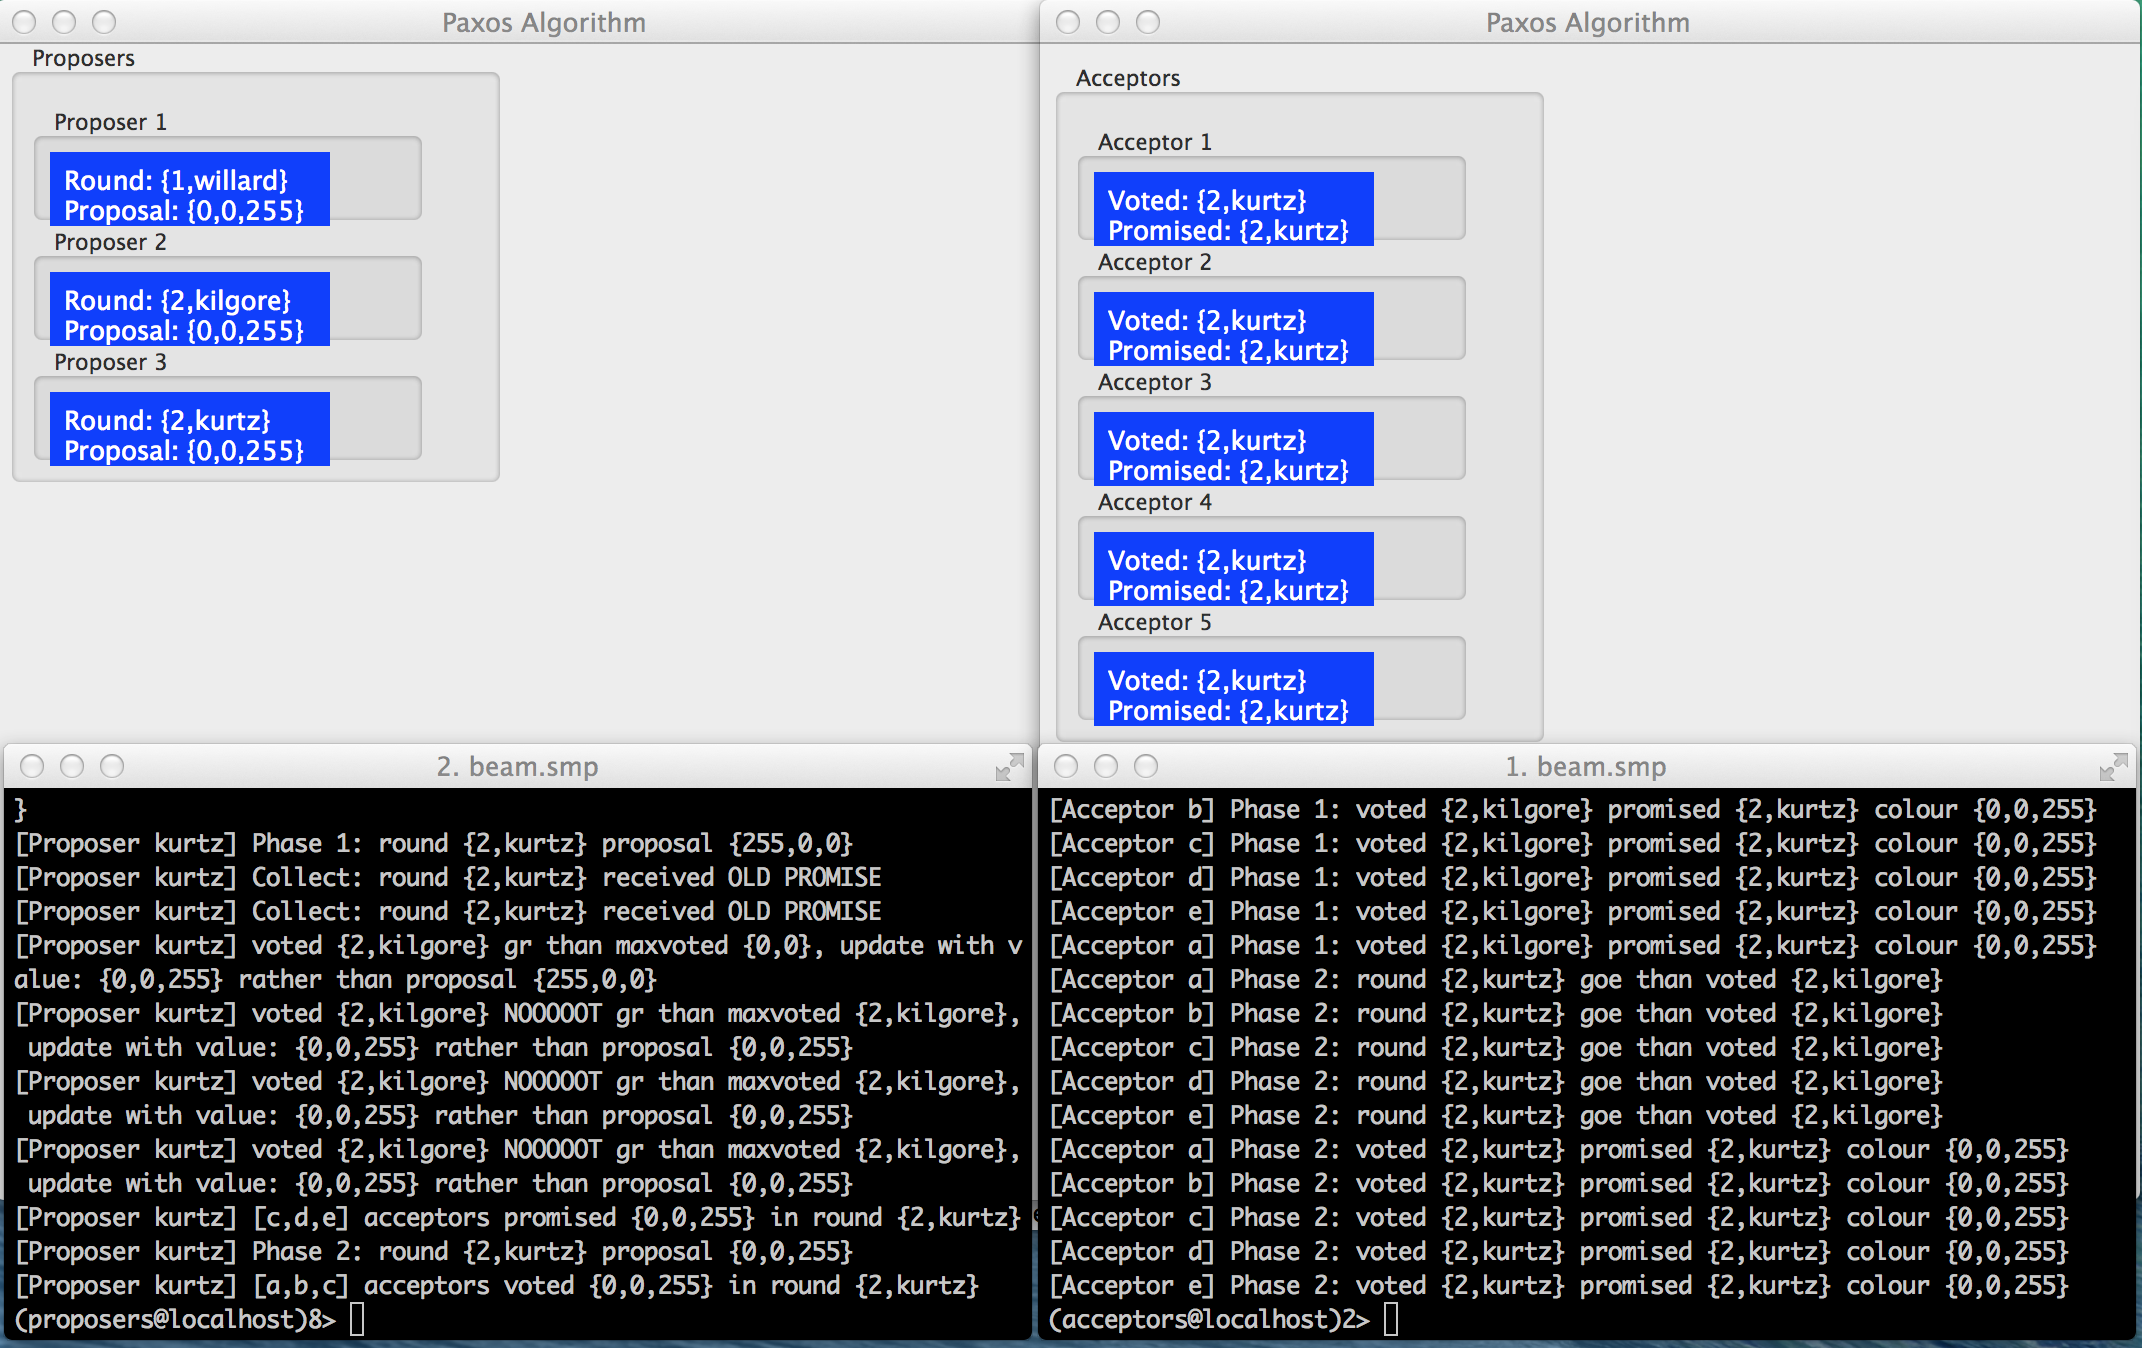
\includegraphics[scale=0.30]{images/exp9.png} \\\\
\newpage

\subsection{Fault Tolerance}

In order to test the fault tolerance we added the \textit{crash} function in the \textit{paxy} module and while running the experiment, we crashed one of the acceptors. Analyzing the trace we see that the acceptor starts again and continues to participate and the algorithm terminates. We ran the experiment both on the same machine and on separate machines for the proposers and acceptors.\\

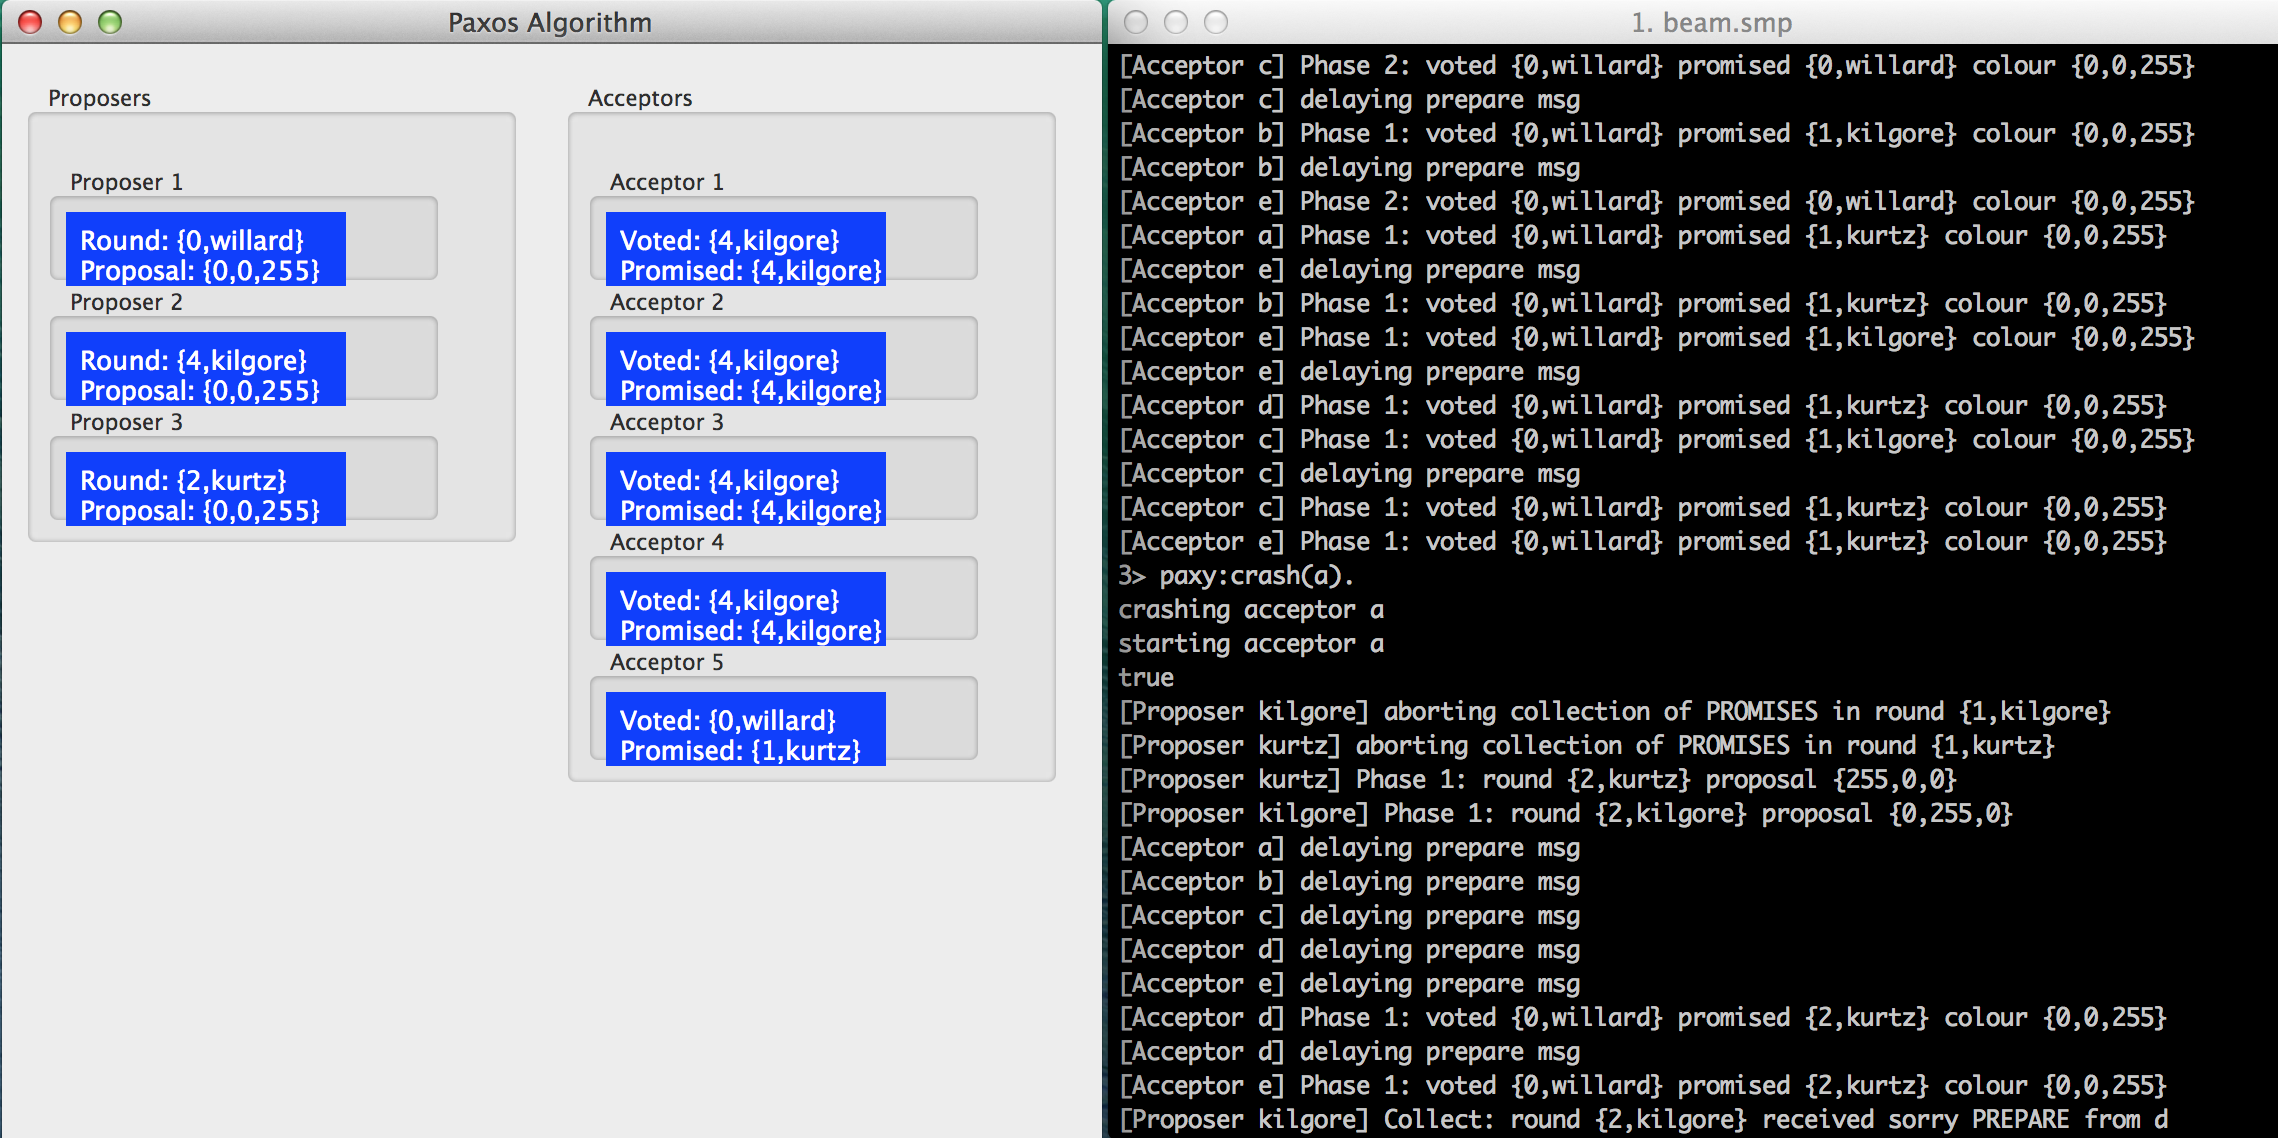
\includegraphics[scale=0.35]{images/exp10.png} \\\\

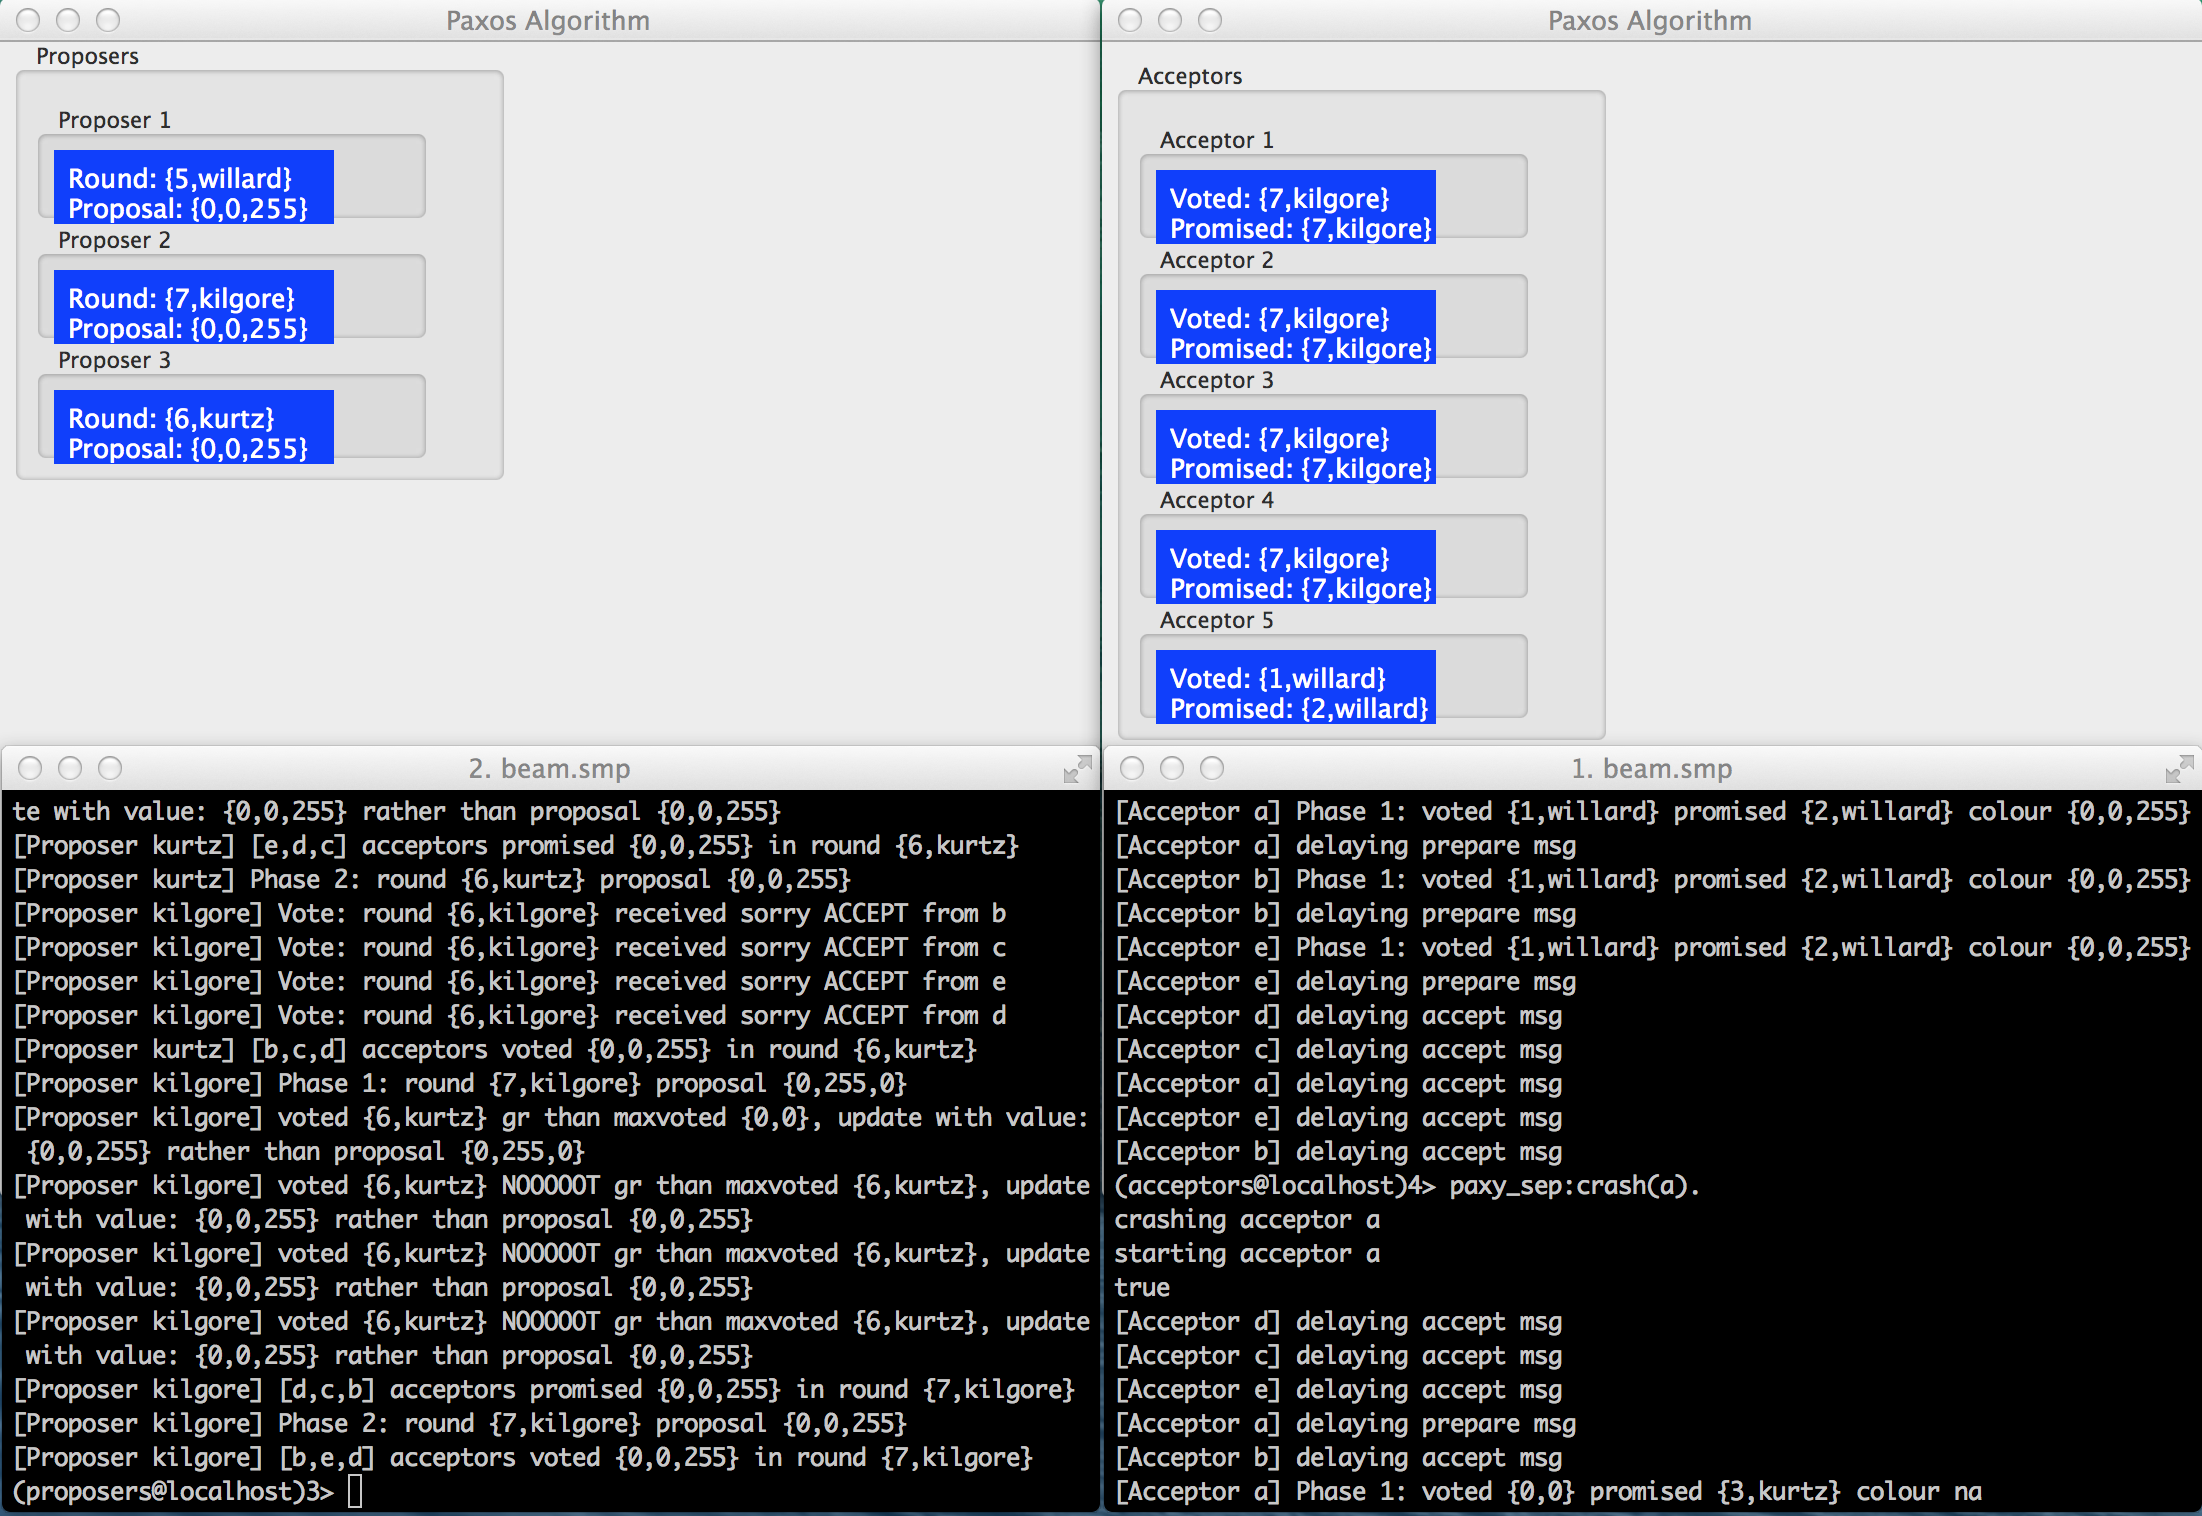
\includegraphics[scale=0.35]{images/exp11.png} \\\\

\subsection{Improvements}

With five acceptors, a proposal needs to be voted on at least 3 times. We changed the \textit{collect} and \textit{vote} functions in the \textit{proposer} module, such that once it receives 3 \textit{sorry} messages it aborts for this proposal. In the experiments trace we see the count of the \textit{sorry} messages and the moment it aborts.\\

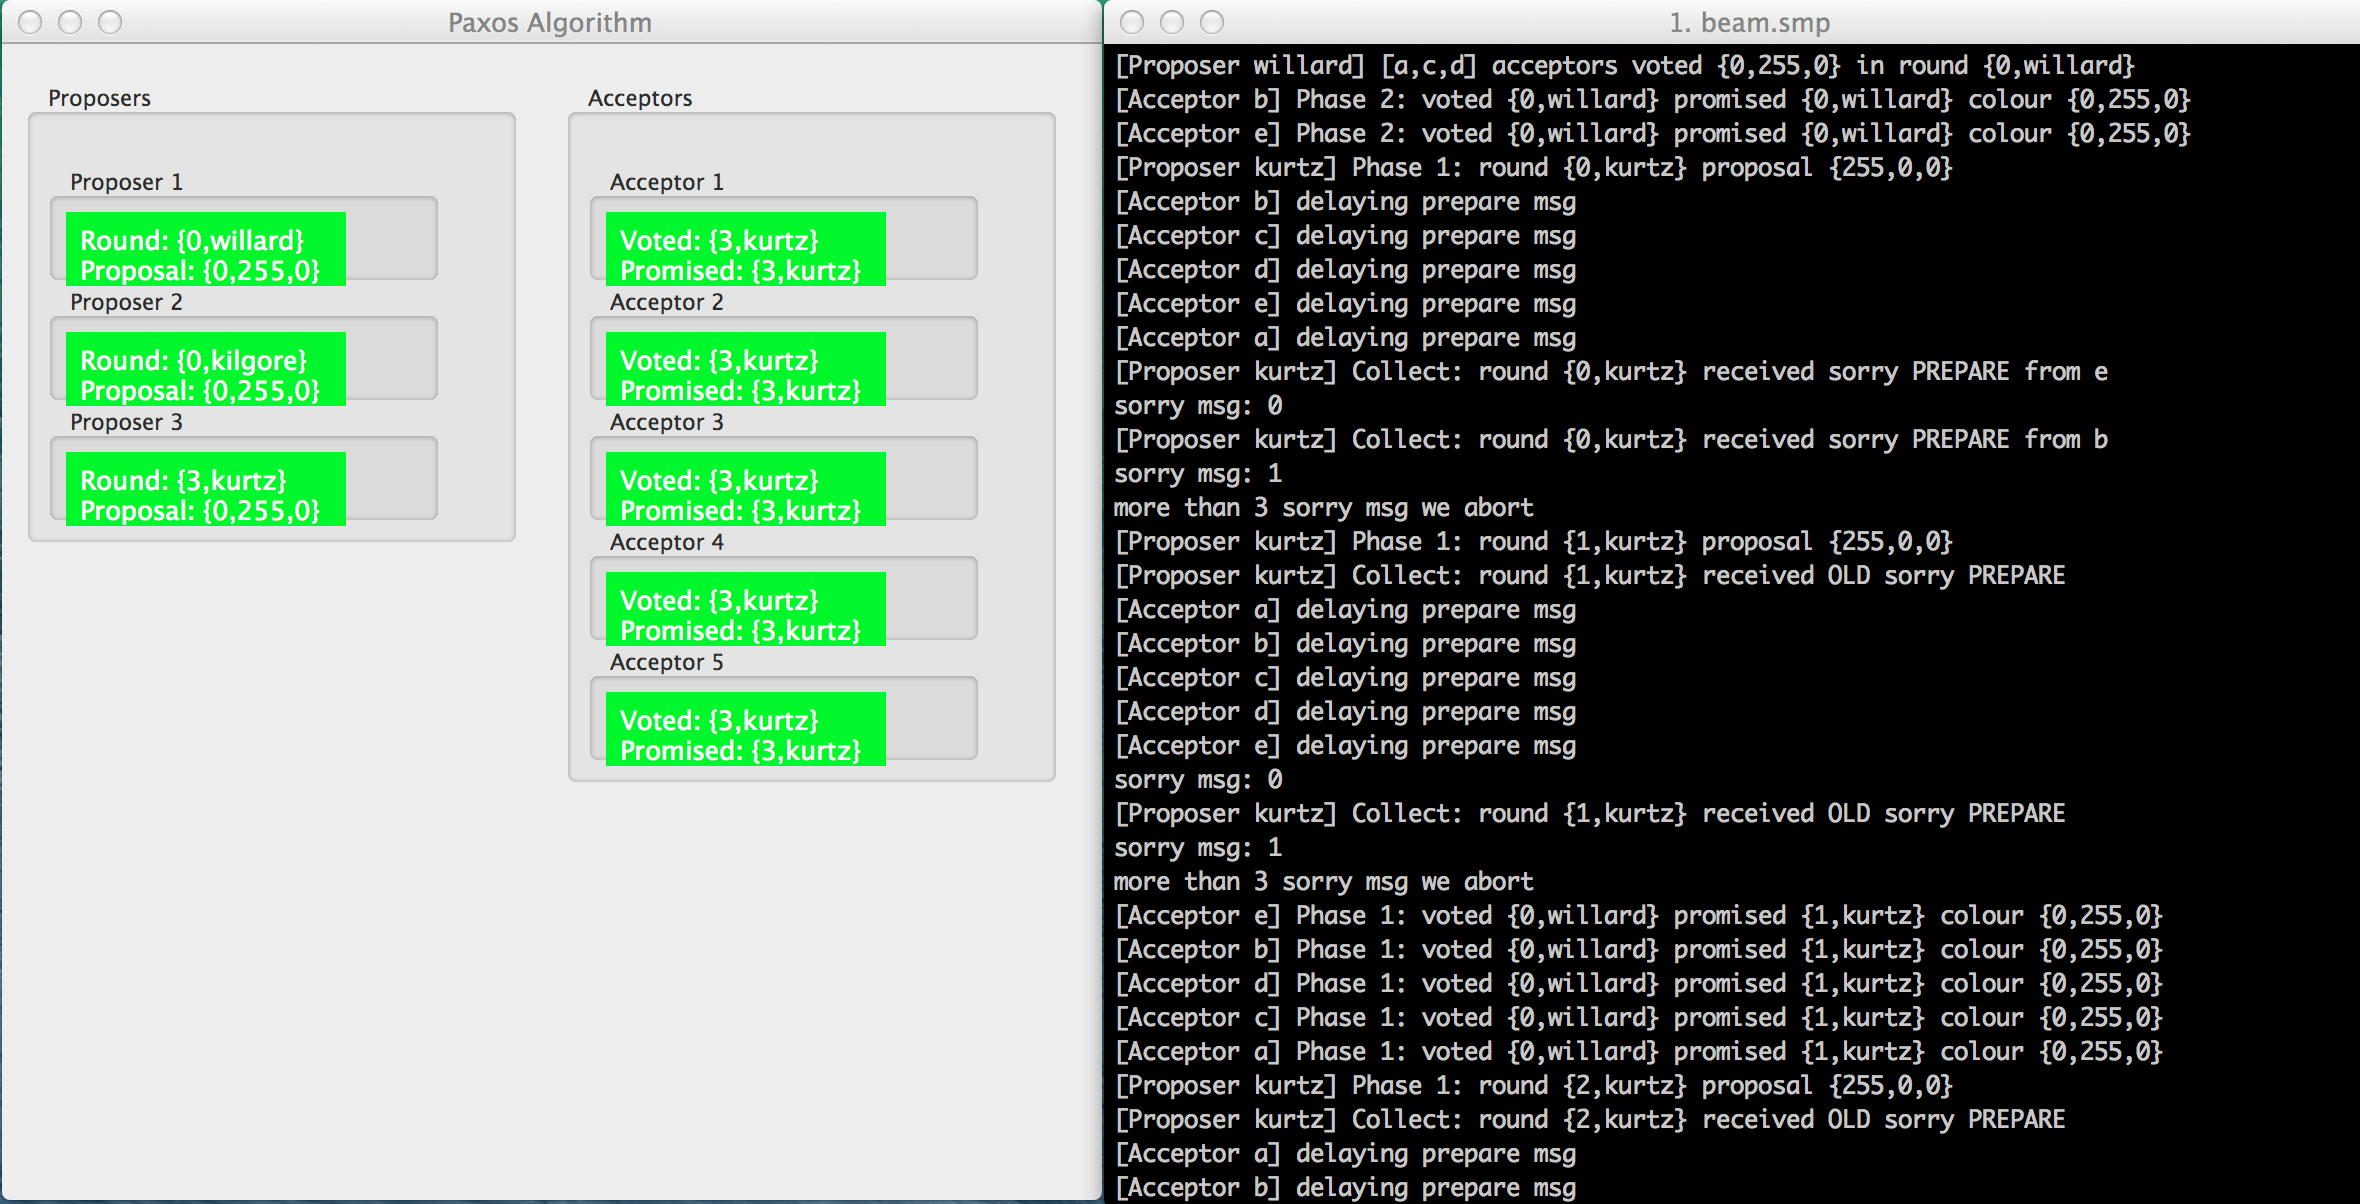
\includegraphics[scale=0.35]{images/exp12.png} \\\\

\section{Personal Opinion}

The seminar had the right level of difficulty for this course and the amount of time available to us. We also got a broader understanding of the \textit{Paxos} algorithm and we managed to run it locally as well as in a distributed system. We are aware that this implementation could have several improvements and modifications as described in the \textit{Leslie Lamport} paper. For instance the algorithm can be extended to work with a group of \textit{learners} processes, and ultimately it can run in a group of servers where each server can play all three roles.

\end{document}
